%\section{Implementation}
\section{Fundamentals of Deep Learning}

The manner in which people gain specific kinds of information, deep learning is that sort of AI and ML to impersonate. While conventional AI computation are straight, deep learning calculations are stacked in an order of expanding intricacy and deliberation. [23].
Neural Networks are basically made-up of several units which work mimicking the human brain’s neurons. Each neuron is connected to another one in order to generate a particular problem to solve. These neurons in AI are called units.
The input layer is the very first neuron of an Artificial brain. It takes raw data from the dataset and passes it to the next-level neurons. And the layer which produces the final output is called the output layer. N total of group may be composed by these input and output layers. Moreover, output layers’ units may depend on the output layer classes. In between these two layers, there can be N numbers of hidden layers, each containing its own weights and biases so that it can calculate its next neuron’s journey. The given density of the network is duplicated to its comparing info and afterward added up bringing about a weighted total, on which the initiation work suggests and delivers the actuation for that neuron, which is without a doubt the result of the neuron signified by y. Then, an activation function will get triggered as an output for this y.


\vspace{5mm}
\begin{figure}[hbt!]
\centering
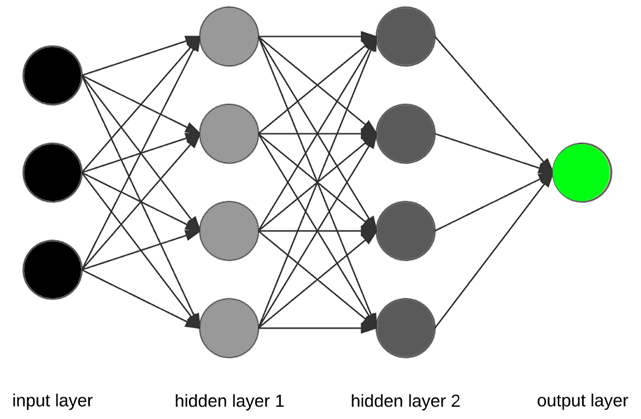
\includegraphics[scale=0.3]{images/fig-4.png}
\caption{Hidden Layer Between Input and Output Layers}
\label{fig:x Hidden Layer Between Input and Output Layers}
\end{figure}

\section{Dataset, Libraries, and Tools}
As our data are mostly direct fundus images from LAG-Dataset[24]. CNN is being used in this thesis for image classification, as it is a type of model which processes data such as images. Also, it automatically understands low-to high-level patterns of image classification. which helps us to extract higher representations for the image content.

\vspace{5mm}
\begin{figure}[htbp]
\centering
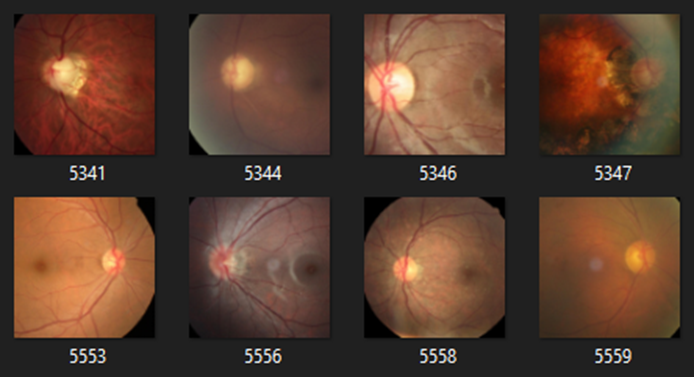
\includegraphics[scale=1]{images/fig-5.png}
\caption{Sample Data form LAG-Dataset}
\label{fig:x Sample Data form LAG-Dataset}
\end{figure}

\noindent This dataset contains 4250 images for \textbf{training}, 302 images for \textbf{testing} and 302 images for \textbf{validation}. All of these folders have two folders for glaucoma and non-glaucoma. The label for “glaucoma” is 1 and for “non-glaucoma” is 0.

\vspace{5mm}
\begin{table}[htbp]
\centering
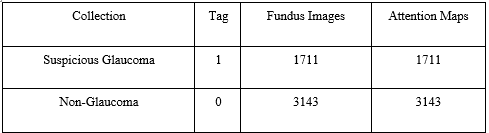
\includegraphics[scale=1]{images/fig_6.png}
\caption{\label{tab:Dissemination of data with tags}Dissemination of data with tags}

% \label{fig:x Dissemination of data with tags }
\end{table}

\noindent In this study, we are going to use the \textbf{python} for coding which is a high level Object Oriented Programming language that has a lot of amazing Machine learning libraries.

\vspace{5mm}
\noindent For this research we are using :

\begin{itemize}
    \item IDE (Google Colab & Jupyter Notebook)
    \item GPU (GTX 1660 super OC)
\end{itemize}

\newpage
\noindent Some of the Libraries that we are going to use are :

\vspace{5mm}
\noindent \textbf{TensorFlow}: TensorFlow is an endways open-source platform for AI that has a far reaching, adaptable biological system of instruments, libraries, and networks [17].

\vspace{5mm}
\noindent \textbf{Keras}: Keras is the prominent Programming interface of TensorFlow 2: a receptive, highly productive point of interaction for taking care of AI issues [18]

\vspace{5mm}
\noindent \textbf{Matplotlib}: Matplotlib is an extensive library for making fixed, energized, and intuitive representations in Python. [25]

\vspace{5mm}
\noindent \textbf{Pandas}: Pandas is an open-source, BSD-authorized library giving elite execution, simple to-utilize information designs, and information reasoning mechanism for Python programming [26]

\vspace{5mm}
\noindent \textbf{Numpy}: NumPy offers thorough numerical actions, random number generators, direct variable-based math schedules, Fourier changes, etc. [19]

\vspace{5mm}
\noindent \textbf{Scikit-Learning}: Straightforward and proficient devices for prescient information investigation Available to everyone, and reusable in different settings · Based on NumPy, SciPy, and matplotlib [27]

\section{Architecture of the Proposed Model}
A class of artificial neural structure which is most commonly enforced to analyze visual imagery is termed as deep learning or a convolutional neural network (CNN, or ConvNet) [20].

\vspace{5mm}
\noindent Transfer Learning approach is proposed in this study. Data set’s size and features provide a perfect environment for implementing a transfer learning approach, allowing a upskilled CNN with all of its density to be utilized to develop a new transfer learning model specialized to identifying Glaucoma with a high degree of accuracy.


\vspace{5mm}
\begin{figure}[hbt!]
\centering
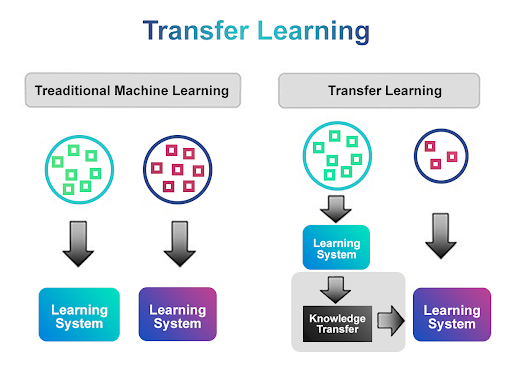
\includegraphics[scale=0.75]{images/fig-7.png}
\caption{Sample Data form LAG-Dataset}
\label{fig:x Sample Data form LAG-Dataset}
\end{figure}

\vspace{5mm}
\noindent We are going with the Fine-Tuning approach of Transfer Learning.

\vspace{5mm}
\noindent The CNN Models we are using are:

\begin{itemize}
    \item VGG-16
    \item InceptionV3
    \item VGG-19
    \item ResNet50
    \item DenseNet121
\end{itemize}

\subsection{VGG-16}
With 16-19 layers of density and little convolution strainers of (33), the VGG [29] Convolutional Neural Network worked by Visual Geometry Group, the University of Oxford has accomplished astounding outcomes. ReLU non-directly is utilized here for invisible layers.

\vspace{5mm}
\noindent In figure 5.4 we can visualize the planning of the VGG-16 model.


\vspace{5mm}
\begin{figure}[hbt!]
\centering
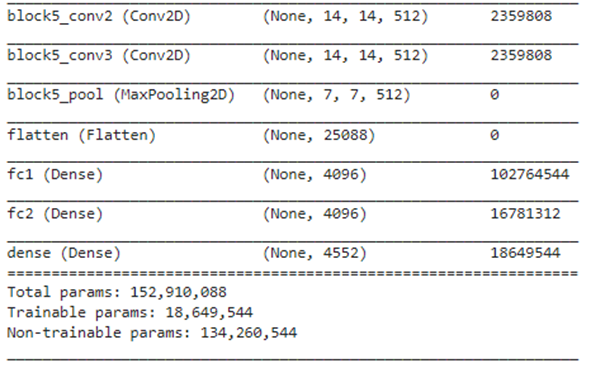
\includegraphics[scale=0.5]{images/fig-8.png}
\caption{Proposed Summary of VGG-16}
\label{fig:x Proposed Summary of VGG-16}
\end{figure}

\vspace{5mm}
\noindent Here we used Keras implementation of VGG-16 model. We used the weights learned from the ImageNet dataset. After downloading the pre-trained model we have made every trained layers into untrainable layers and deleted the top 3 layer layers to reuse the model. Then we use a Flatten layer to flatten every previous models layers into one and we used 3 Dense neurons with 100 layers in each of them. Input shape of our dataset's images are 224 x 224. We used the “ReLU” activation function for the Convolutional layers. For predictions, we used the A Dense neuron with 2 layers in it for 2 output (Glaucoma and Non-glaucoma) and “Softmax” for activation function.

\vspace{5mm}
\noindent In figure 5.5 we can visualize the architecture of the VGG-16  model.

\vspace{5mm}
\begin{figure}[hbt!]
\centering
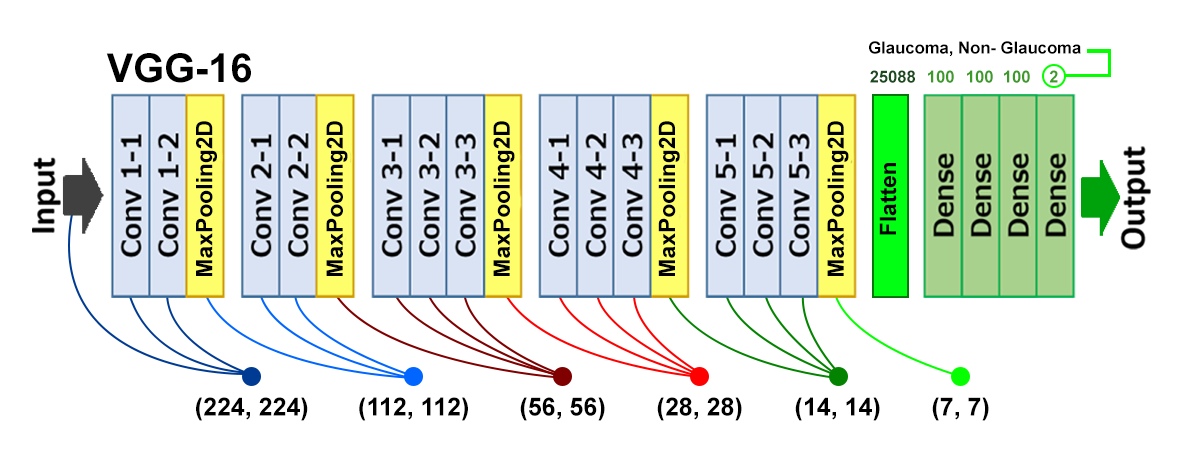
\includegraphics[scale=0.75]{images/Architecture of VGG-16.png}
\caption{Architecture of VGG-16}
\label{fig:x Architecture of VGG-16}
\end{figure}

\subsection{Inception V3}
The Inception [30] architecture is made up of several inception modules stacked on top of each other to form a deep neural network, where the inception modules provide the ability to work them all in equal and link their results into a solitary result vector for contribution to the module a short time later.

\vspace{5mm}
\noindent In figure 5.6 we can visualize our model summary of InceptionV3.

\vspace{5mm}
\begin{figure}[hbt!]
\centering
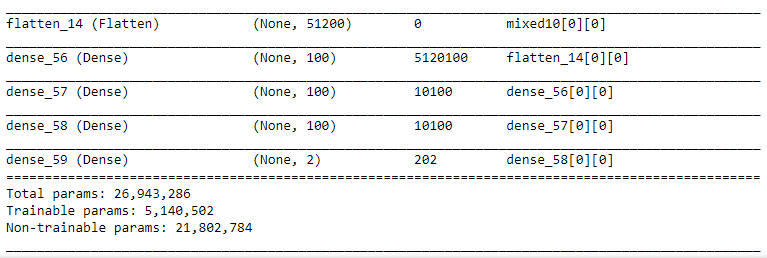
\includegraphics[scale=0.75]{images/fig-11.png}
\caption{Model Summary of InceptionV3}
\label{fig:x Model Summary of InceptionV3}
\end{figure}

\vspace{5mm}
\noindent Here we used Keras implementation of InceptionV3 model. We used the weights learned from the ImageNet dataset. After downloading the pre-trained model we have made every trained layers into untrainable layers and deleted the top 3 layer layers to reuse the model. Then we use a Flatten layer to flatten every previous models layers into one and we used 3 Dense neurons with 100 layers in each of them. Input shape of our dataset's images are 224 x 224. We used the “ReLU” activation function for the Convolutional layers. For predictions, we used the A Dense neuron with 2 layers in it and “Softmax” for activation function.

\subsection{VGG-19}
VGG19 is a variation of the VGG model which in short comprises of 19 layers (16 convolution layers, 3 completely associated layers, 5 MaxPool layers, and 1 SoftMax layer). [32] VGG19 has 19.6 billion Failures. In Figure 5.7, Our model summary for VGG-19 is given.

\vspace{5mm}
\begin{figure}[hbt!]
\centering
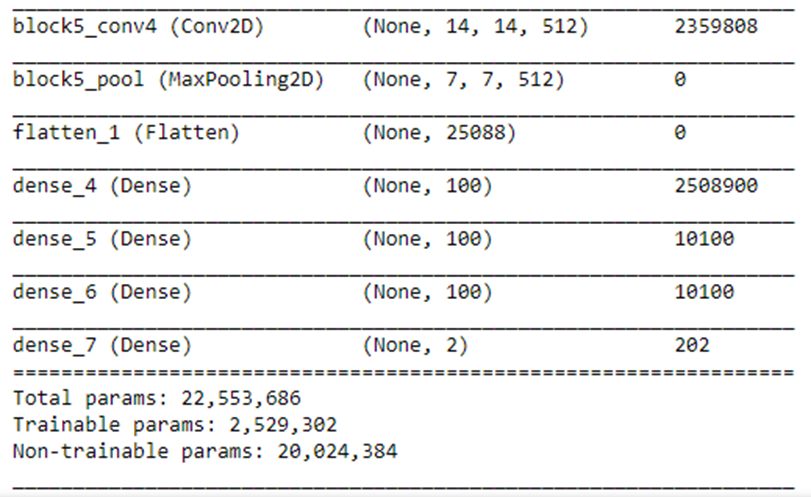
\includegraphics[scale=1]{images/fig-12.png}
\caption{Model Summary of VGG-19}
\label{fig:x Model Summary of VGG-19}
\end{figure}

\vspace{5mm}
\noindent Here we used Keras implementation of VGG-19 model. We used the weights learned from the ImageNet dataset. After downloading the pre-trained model we have made every trained layers into untrainable layers and deleted the top 3 layer layers to reuse the model. Then we use a Flatten layer to flatten every previous models layers into one and we used 3 Dense neurons with 100 layers in each of them. Input shape of our dataset's images are 224 x 224. We used the “ReLU” activation function for the Convolutional layers. Then we performed batch normalization used a dropout rate of 0.5. In Figure 5.8, Our model summary for VGG-19 is given.

\vspace{5mm}
\begin{figure}[hbt!]
\centering
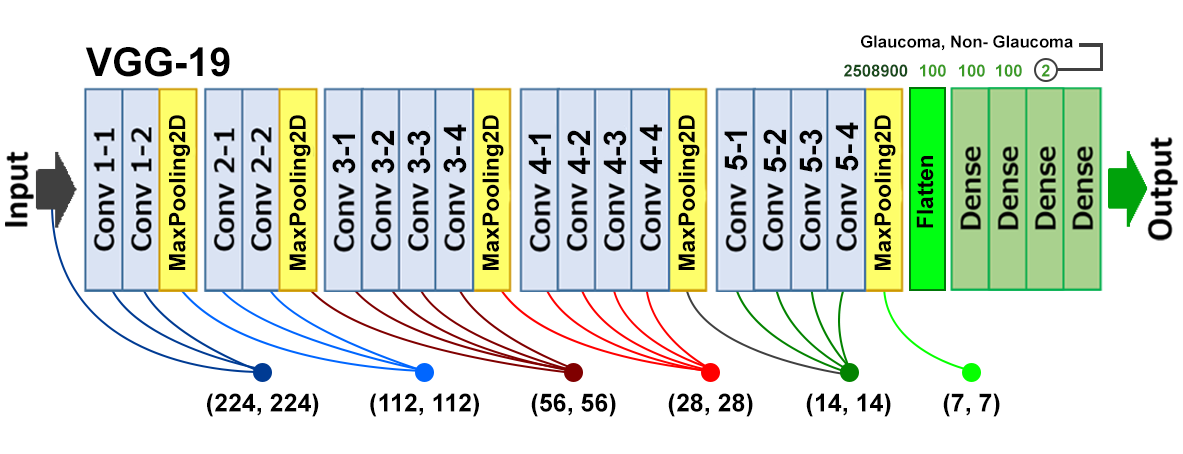
\includegraphics[scale=0.75]{images/Architecture of VGG-19.png}
\caption{Architecture of VGG-19}
\label{fig:x Architecture of VGG-19}
\end{figure}

\vspace{5mm}
\noindent For expectations, we involved the A Thick neuron with 2 layers in it and "Softmax" for initiation work. For the Angle Drop, we utilized the Adam enhancer with a learning pace of \(10^-5\).

\subsection{ResNet50}
ResNet50 is a variant of the ResNet model which has 48 convolution layers and 1 MaxPool layer and 1 normal pool layer. Besides, it has 3.8 x 109 floating point activities. ResNet50 assumes a significant part in the computer vision and profound learning world. It is principally utilized for picture acknowledgment and is most ordinarily applied for dissecting visual symbolism. Additionally, it is a pre-prepared Profound Learning model for picture order of the Convolutional Neural Organization (CNN).  ResNet50 is mainly trained on a million images of 1000 categories from the ImageNet database and there are over 23 million trained parameters which will make it more suitable for image recognition. ResNet50 is deeper than any other network using residual connections. In Figure 5.9, we can visualize the architecture of a ResNet50 model.

\vspace{5mm}
\noindent In Figure 5.9, we can visualize the architecture of a ResNet50 model.

\vspace{5mm}
\begin{figure}[hbt!]
\centering
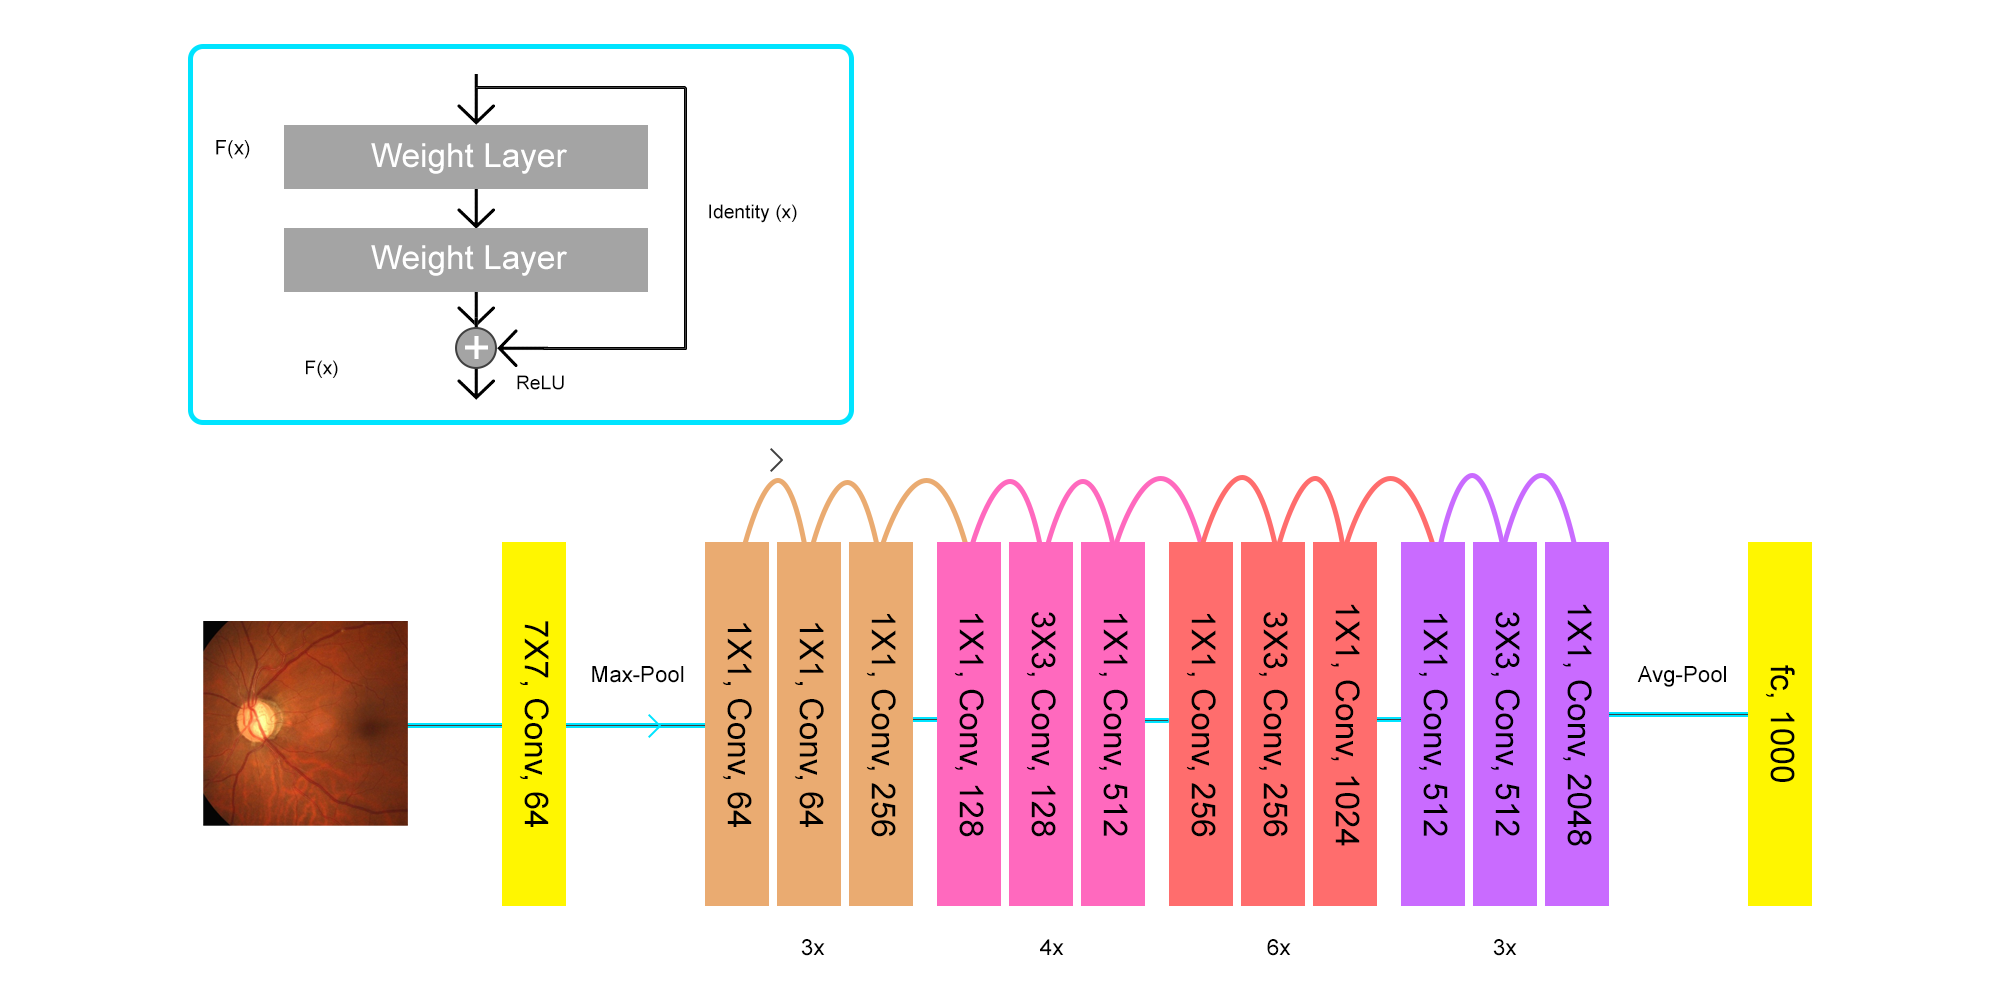
\includegraphics[scale=0.45]{images/resnet50.png}
\caption{Architecture of ResNet50}
\label{fig:x Model Summary of ResNet50}
\end{figure}

\vspace{5mm}
\begin{figure}[hbt!]
\centering
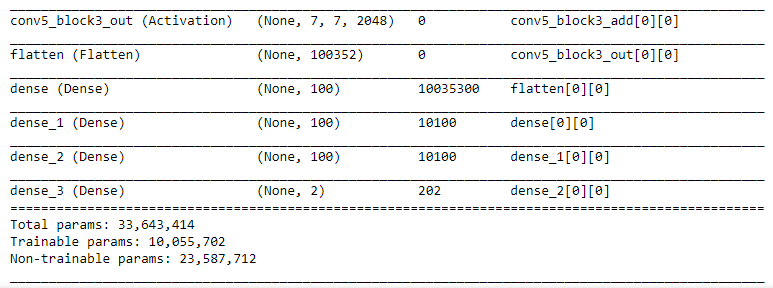
\includegraphics[scale=0.7]{images/ResNet50.PNG}
\caption{Model Summary of ResNet50}
\label{fig:x Model Summary of ResNet50}
\end{figure}

\vspace{5mm}
\noindent Here, we used the Keras implementation of the ResNet50 Model. We used the weights learned from the ImageNet dataset. After downloading the pre-trained model we have made every trained layers into untrainable layers and deleted the top 3 layer layers to reuse the model. Then we use a Flatten layer to flatten every previous models layers into one and we used 3 Dense neurons with 100 layers in each of them. Input shape of our dataset's images are 224 x 224. We used the “ReLU” activation function for the Convolutional layers. For predictions, we used the A Dense neuron with 2 layers in it and “Softmax” for activation function. 



\subsection{DenseNet121}
Dense Convolutional Network which is DenseNet is a design that bright lights on making the significant learning networks go impressively more significant, but making them more capable to get ready, by using more restricted relationship between the layers [33]. DenseNet is actually similar to ResNet for specific key differentiations. For example, ResNet uses an additional substance system that consolidates the former layer with the future layer, while DenseNet joins the consequence of the first layer with the future layer. This is done to enable the best information stream between the layers of the association.

\vspace{5mm}
\begin{figure}[hbt!]
\centering
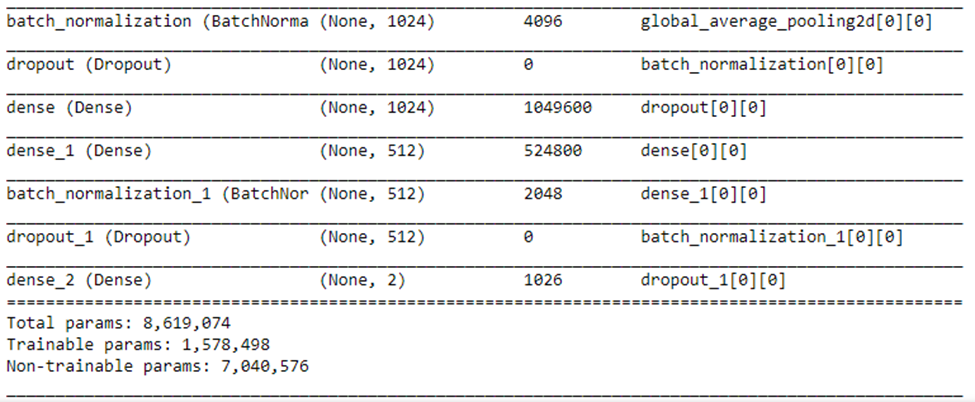
\includegraphics[scale=0.5]{images/fig-15.png}
\caption{Model Summary of DenseNet121}
\label{fig:x Model Summary of DenseNet121}
\end{figure}
\vspace{5mm}

\vspace{5mm}
\begin{figure}[hbt!]
\centering
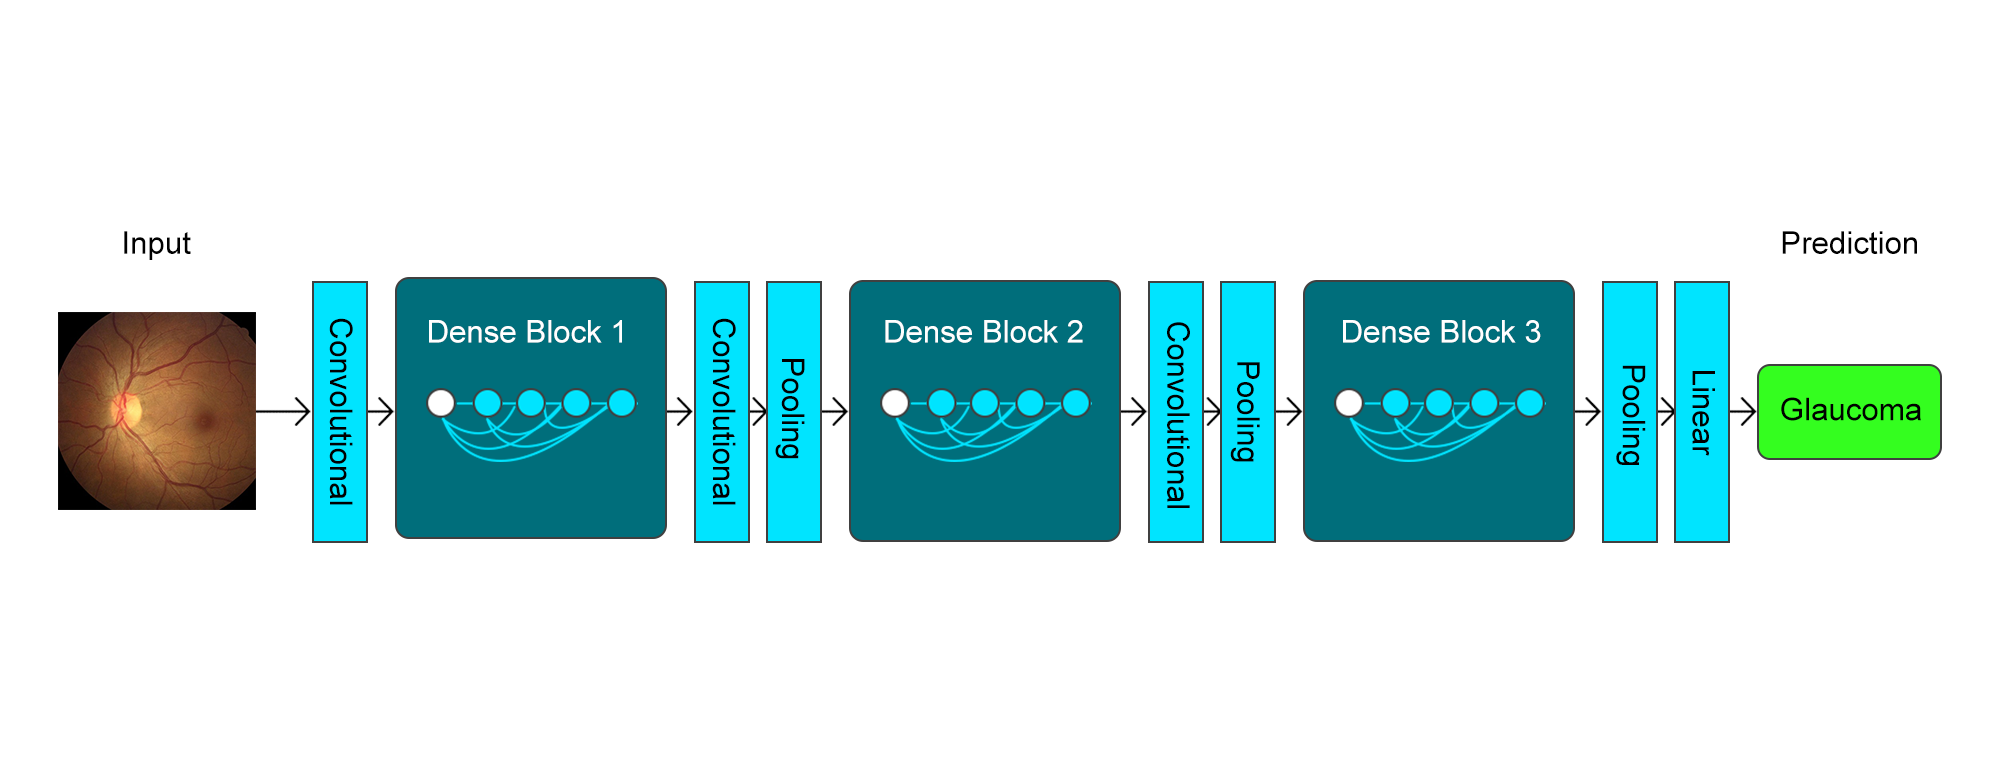
\includegraphics[scale=0.4]{images/densenet archinew.png}
\caption{Architecture of DenseNet121}
\label{fig:x Model Summary of DenseNet121}
\end{figure}
\vspace{5mm}

\noindent Here, we used the Keras implementation of the DenseNet121 model . We used the weights learned from the ImageNet dataset. After downloading the pre-trained model we have made every trained layers into untrainable layers and deleted the top 3 layer layers to reuse the model. Then we use a Flatten layer to flatten every previous models layers into one and we used 3 Dense neurons with 1024 layers, 512 layers and 256 layers in each of them. Input shape of our dataset's images are 224 x 224. We used the “ReLU” activation function for the Convolutional layers. For predictions, we used the A Dense neuron with 2 layers in it and “Softmax” for activation function.



\section{Fine Turing}
Fine-tuning is the process of fine-tuning or changing a model which has previously been trained for one job to make it work as a 2nd task which was related. A deep learning network that recognizes cars, for example, maybe fine-tuned to recognize trucks [25]. As proposed, we will be using Fine-tuning approach to detect Glaucoma from our dataset which will help to detect our wanted result in this study.

\vspace{5mm}
\begin{figure}[hbt!]
\centering
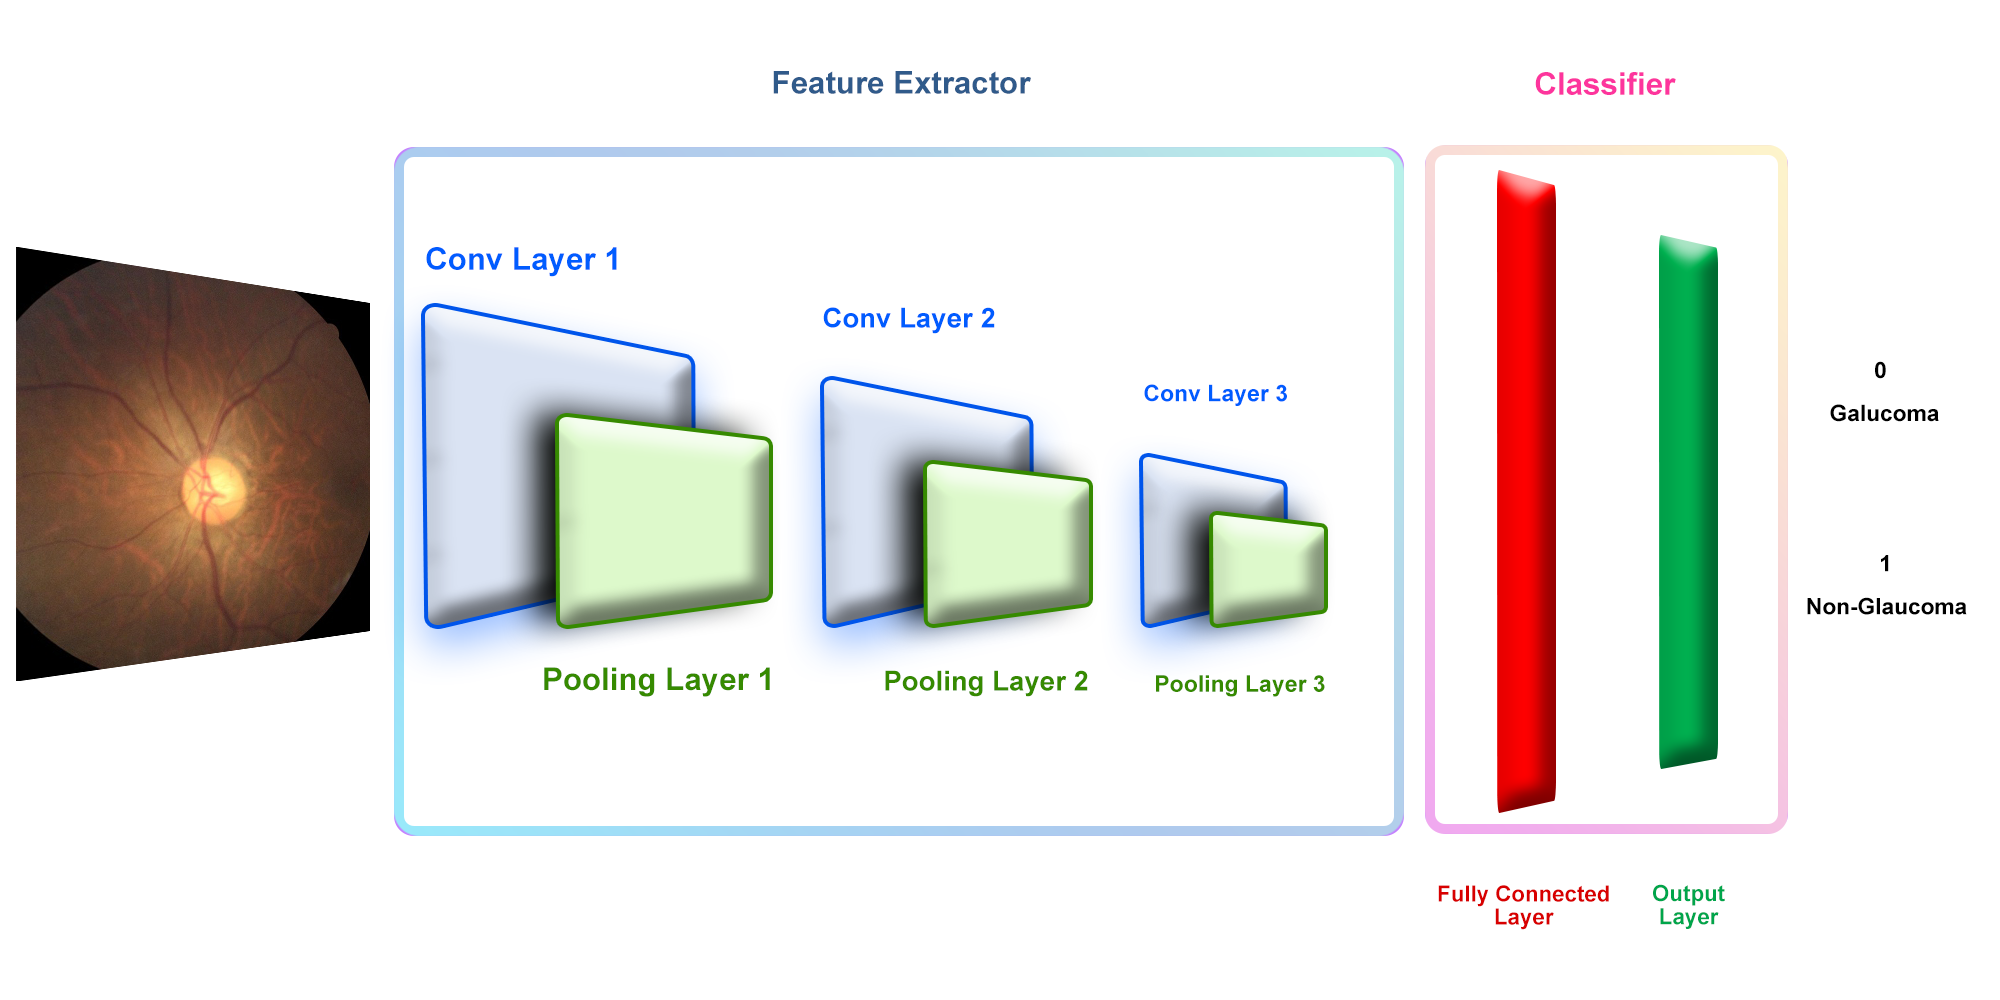
\includegraphics[scale=0.4]{images/Fine-tuning by keeping the feature extractor_s final layers trainable.png}
\caption{Fine-tuning by keeping the feature extractor's final layers trainable}
\label{fig:x Fine-tuning by keeping the feature extractor's final layers trainable}
\end{figure}

\newpage
\subsection{Segments of CNN}

\vspace{5mm}
The architecture of Convolutional Neural Networks is basically 3 types of layers.

\begin{itemize}
    \item Convolutional
    \item Pooling
    \item Fully Connected
\end{itemize}

\vspace{5mm}
\begin{figure}[hbt!]
\centering
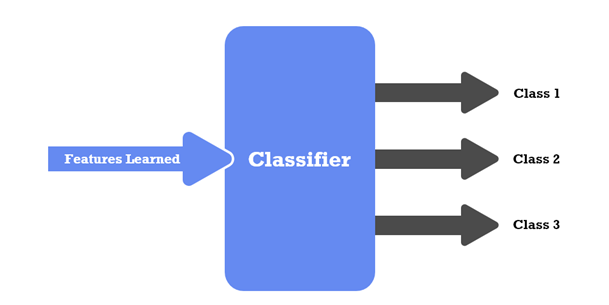
\includegraphics[scale=1]{images/fig-17.png}
\caption{CNN Classifier}
\label{fig:x CNN Classifier}
\end{figure}

\noindent And basically, all these layers do these operations as bellow:

\vspace{5mm}
\begin{itemize}
    \item Convolution operation
    \item Pooling operation
    \item Flattening
    \item Non-linear activation functions imply
    \item Optimization operation
\end{itemize}

\vspace{5mm}
\subsection{Convolutional Operation}


\vspace{5mm}
As illustrated in \textbf{figure 5.15}, the convolutional layers are responsible for convolution operations and create feature maps that learn the characteristics of the image taken as input by convolving correctly learnt filters or kernels with the input array or tensor. \textbf{Figure 5.16} shows how a convolution operation contains a number of feature maps that record new features and respond to feature hierarchy across the neural network, from the early layers to the far edging layers. [29] [34] [30]

\vspace{5mm}
\begin{figure}[hbt!]
\centering
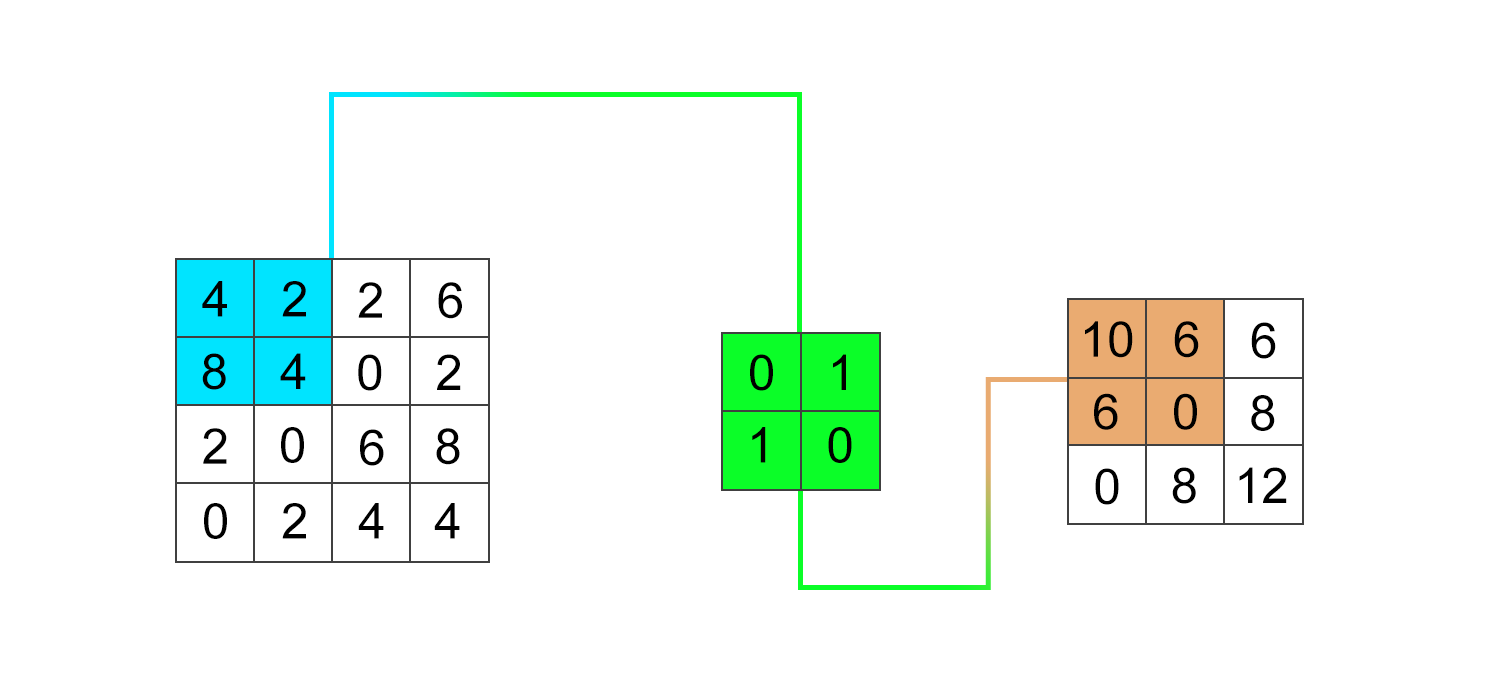
\includegraphics[scale=0.5]{images/feature map.png}
\caption{Convolution Operation}
\label{fig:x Convolution Operation}
\end{figure}

\vspace{5mm}
\begin{figure}[hbt!]
\centering
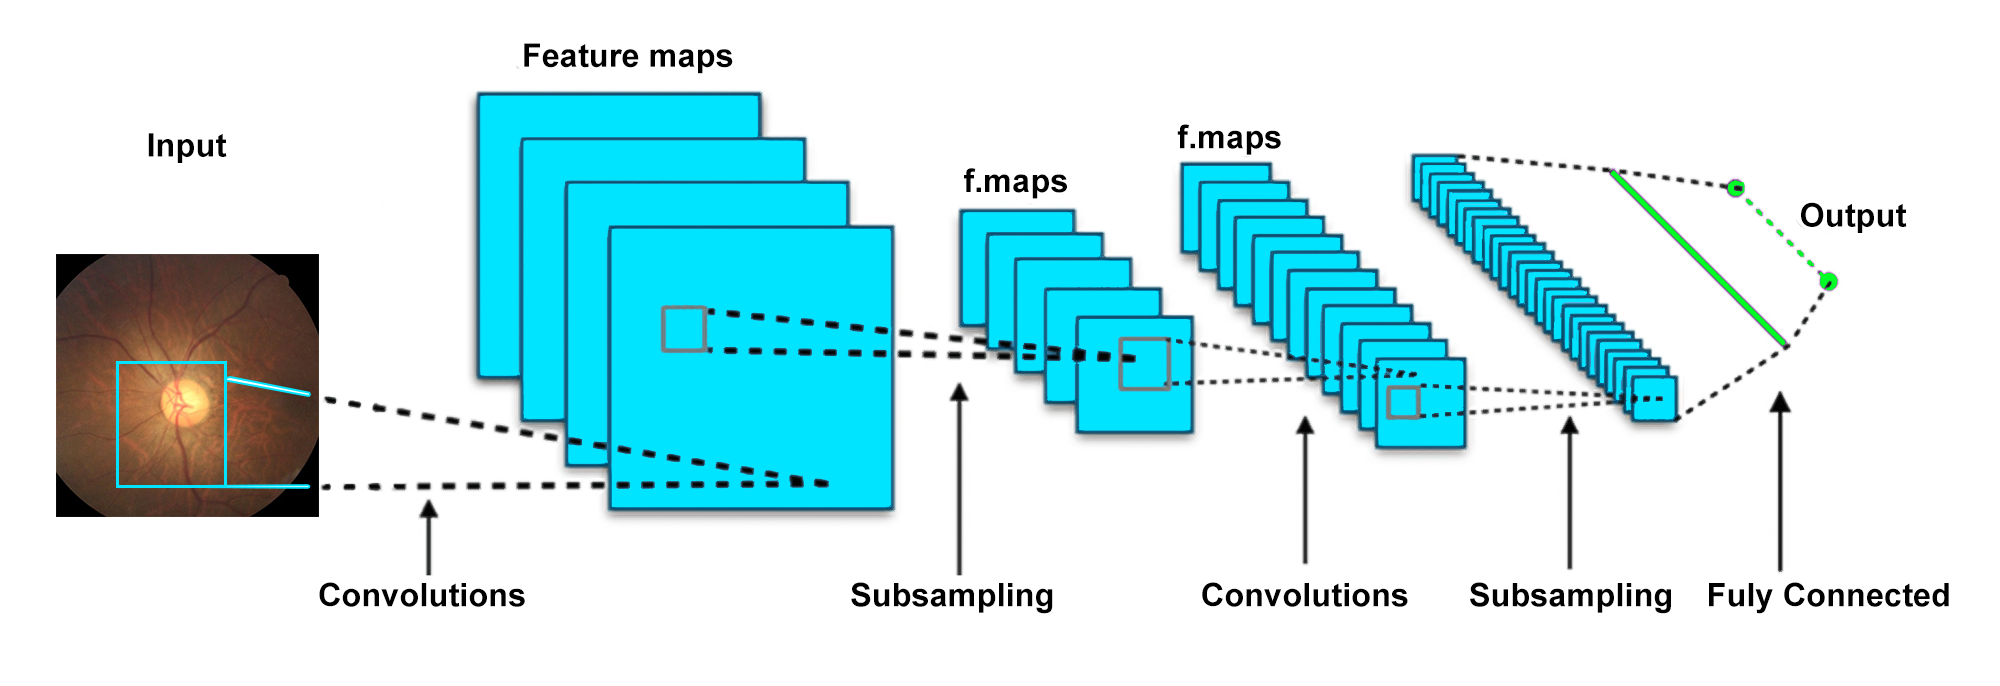
\includegraphics[scale=0.4]{images/planes shown are a feature map.png}
\caption{Feature map}
\label{fig:x Feature map}
\end{figure}

\newpage
\subsection{Pooling Operation}

\vspace{5mm}
The feature maps are pooled in order to extract more features and minimize their dimension[30]. In general, the pooling operation is carried out as follows:
\vspace{5mm}
\begin{figure}[hbt!]
\centering
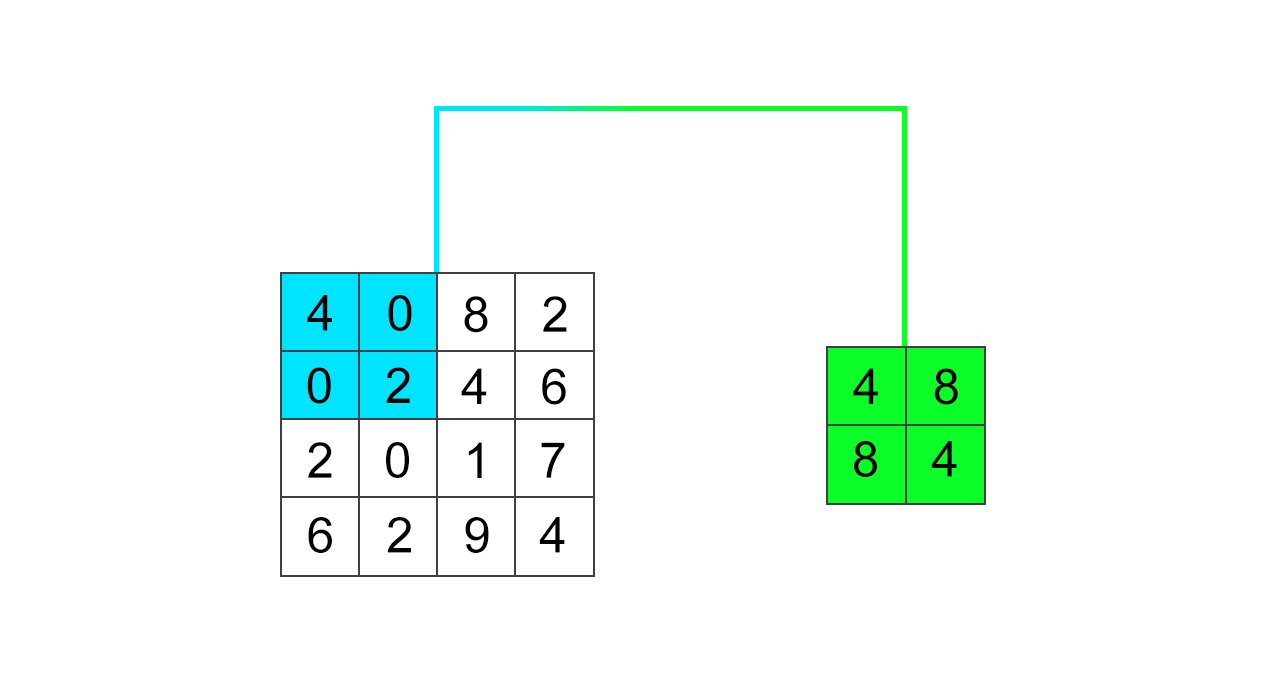
\includegraphics[scale=0.5]{images/pooling.png}
\caption{Pooling Operation}
\label{fig:x Pooling Operation}
\end{figure}
\vspace{5mm}
\begin{itemize}
    \item \textbf{Max Pooling}: As an output, the greatest value of a patch of numbers from the feature map that was utilized as input is returned. [30]
    \item \textbf{Average Pooling}: It produces the average as an output, the value of the patch of digits from the feature map that's been utilized as an input. [34]
    \item \textbf{GlobalAveragePooling2D}: GlobalAveragePooling2D takes a new approach. The spatial dimensions are average pooled until each spatial dimension is one.
\end{itemize}

\vspace{5mm}
\begin{figure}[hbt!]
\centering
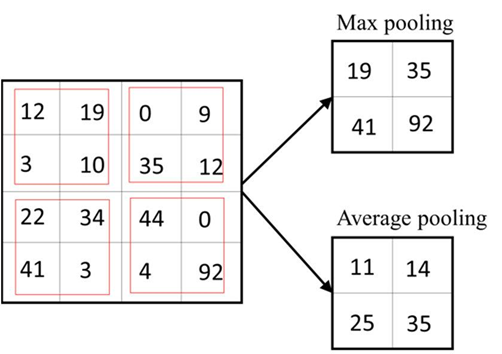
\includegraphics[scale=1]{images/fig-21.png}
\caption{Max and Average Pooling}
\label{fig:x Max and Average Pooling}
\end{figure}

\vspace{5mm}
\subsection{Flattening Layers}

\vspace{5mm}
The process of flattening data into a one-dimensional array for usage in the next layer is known as flattening. To produce a single lengthy feature vector, we flatten the output of a convolutional layers. It's also related to the final categorization model, as a fully-connected layer [35].

\vspace{5mm}
\begin{figure}[hbt!]
\centering
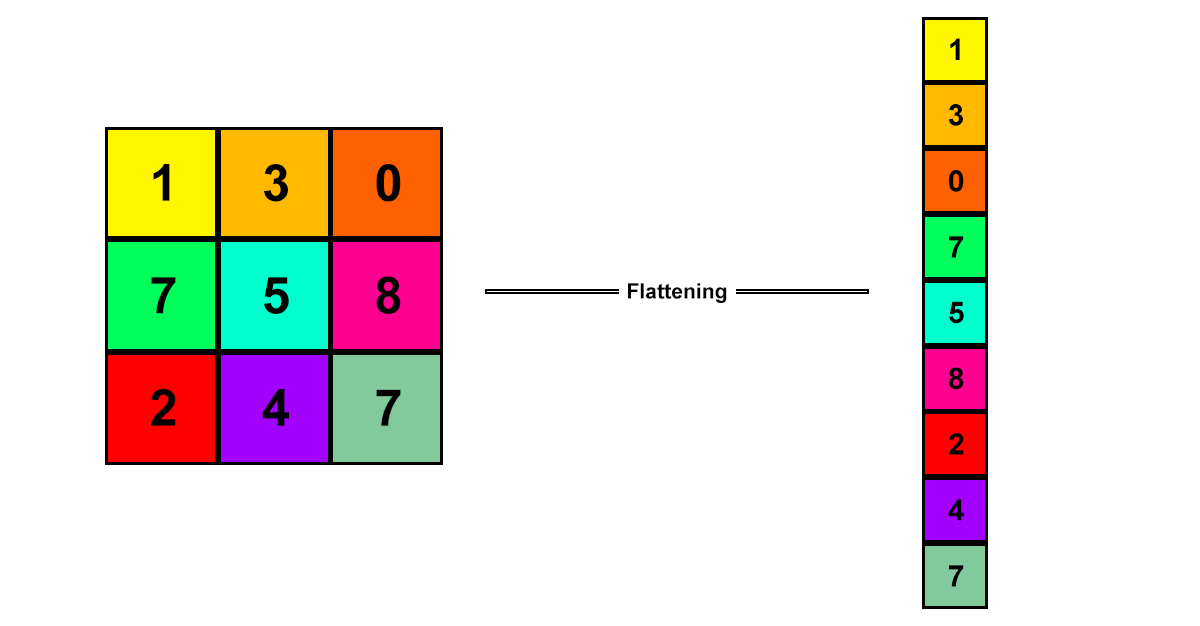
\includegraphics[scale=0.5]{images/Pooling Matrix to Flattening..png}
\caption{Pooling Matrix to Flattening.}
\label{fig:x Pooling Matrix to Flattening}
\end{figure}

\vspace{5mm}
\subsection{Fully Connected Layers}

\vspace{5mm}
Fully linked layers in a neural network are those where all of the inputs through one layer are connected with every activation unit of next layer. In most common machine learning models, these last several layers are fully linked layers that combine the data acquired by previous levels to generate the final output [36].

\vspace{5mm}
\begin{figure}[hbt!]
\centering
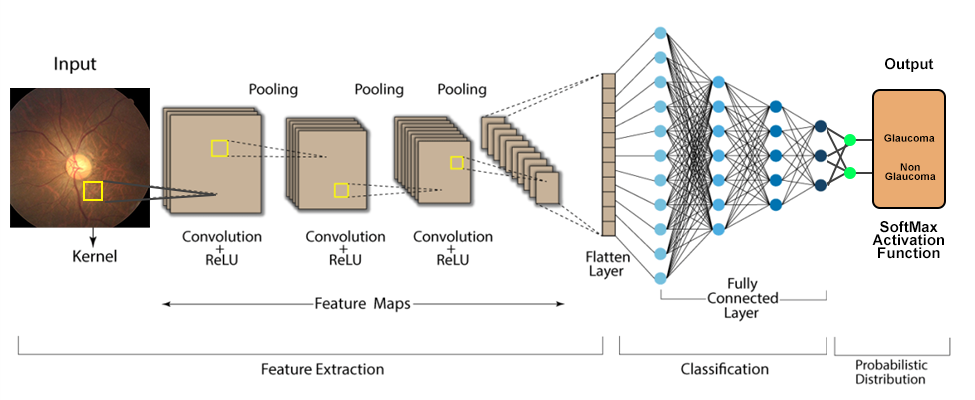
\includegraphics[scale=0.45]{images/Fully Connected CNN classifying between classes.png}
\caption{Classifying different classes using a fully connected CNN}
\label{fig:x Classifying different classes using a fully connected CNN}
\end{figure}

\noindent Fully connected layers or in other words dense layers take nonlinear activation functions, however, the final output layer of the fully connected layers take Softmax activation.

\vspace{5mm}
\noindent We are also going to use SoftMax and ReLU in both VGG-16 and InceptionV3.

\vspace{5mm}
\subsection{Optimization Algorithm}
\vspace{5mm}
\noindent When deep learning is utilized for training, an optimization technique is applied to improve the cost function. This algorithm's general equation is as follows:

\vspace{5mm}
\begin{equation*}
J(W,\ b) = \frac{1}{m}\sum_{i=1}^m\ L(y^{'i},y^i)
\end{equation*}

\vspace{5mm}
\noindent We applied Adam optimizer in our models, which would be discussed below: Algorithm Adam is a well-known algorithm that is noted for the speed it contains. Adaptive Momentum is the abbreviation for AdaM. At the same time, Adam associates the propulsion RMSprop. As a result, Adam is a highly powerful and quick algorithm. This approach is relatively straightforward in its implementation, quite efficient in estimate, and uses very little memory. For larger issues with data or parameters, it is more efficient. The optimizer is defined by the equations below:

\vspace{5mm}
\begin{equation*}
\begin{split}
\alpha_t = \alpha.\frac{\sqrt{1-\beta^t_2}}{1-\beta^t_2} \\
\theta_t\leftarrow\theta_{t-1}-\alpha_t-.m_{\frac{t}{(\sqrt{v_t}+\hat{\epsilon})}}
\end{split}
\end{equation*}
\vspace{5mm}
For the Gradient Descent, we used the Adam optimizer with a learning rate of 10-5. 

\vspace{5mm}
\subsection{Softmax}
\vspace{5mm}
\noindent The output of this function is a probability distribution. As the entire summation becomes 1, it maps the input. This function is defined by the equation given below:

\vspace{5mm}
\begin{equation*}
f_j(z)=\frac{e^{zj}}{\sum_k{e^zk}} 
\end{equation*}

\vspace{5mm}
\noindent It squashes a vector of arbitrary real-valued scores (in z) into a vector of values between 0 and 1 that add to 1.

\vspace{5mm}
\subsection{Rectified Linear Unit (ReLU)}
\vspace{5mm}
\noindent ReLU is a piecewise linear function that directly outputs the input. It has a 0 to range. In the deep learning era, amongst most well-known activation function ReLU is the one, as seen in below mentioned equation:

\vspace{5mm}
\begin{equation*}
y=max(0,x) 
\end{equation*}

\vspace{5mm}
\noindent ReLU's main advantage is that it solves the vanishing gradient problem, is one-sided (unlike TanH), has sparse activation (50\%) and no back propagation error. This function is monotonic, as are its derivatives. the fact that this function is non-zero centered and non-differentiable by zero is a drawback. Another drawback is the dwindling ReLU population. which occurs when half of the outputs for non-zero centered action are inactive (returned as 0).


\vspace{5mm}
\subsection{Batch Normalization}

\vspace{5mm}
While feeding input to Neural Networks, we do Batch Normalization because it makes the training faster and handles internal covariate shift. Again Normalizing the input for a similar range of values can speed up the learning. Because Batch Normalization normalizes the outputs of the activation functions in every layer of the neural network, not just in the inputs. In their original paper, Sergey et al. [37] claim that it minimizes the network's inner covariate shift. 

\vspace{5mm}
\subsection{Dropout}

\vspace{5mm}
Adulteration of training information misleadingly regulates to over fit through dropout and other characteristically noise systems. Dropout holds out a kind of versatile regularization for summed up straight models [38]. Moreover, Dropout is a normal stochastic choice strategy in view of the neural organization [39]. It causes this level to appear and be handled as a level with a certain measure of hubs and availability in comparison to the previous level. Essentially, a particular perspective on the designed layer is directed with each update to a layer during preparing.

\newpage
\section{Analysis}
We have used VGG-16, VGG-19, DenseNet121, InceptionV3 and ResNet50 models for our study. Every model was compiled with Adam optimizer with the learning rate of 1e-5 in 50 epochs. 

\vspace{5mm}
\noindent After 50 epochs, RestNet50 got the highest score among the other models with a validation accuracy of 94.7\%.

\vspace{5mm}
\noindent These are the Train and Test score of our models - 

\begin{table}[hbt!]
\resizebox{\textwidth}{!}{%
\begin{tabular}{@{}|c|c|c|c|c|c|c|@{}}
\toprule
Model       & \multicolumn{1}{l|}{Epochs} & Accuracy & Train Accuracy & Train Loss & Validation Loss & \multicolumn{1}{l|}{Weight} \\ \midrule
DenseNet121 & \multirow{5}{*}{50}         & 86.81\%  & 88.83\%        & 31.18\%    & 24.10\%         & \multirow{5}{*}{ImageNet}   \\ \cmidrule(r){1-1} \cmidrule(lr){3-6}
InceptionV3 &  & 86.42\% & 93.49\% & 20.04\% & 35.79\% &  \\ \cmidrule(r){1-1} \cmidrule(lr){3-6}
ResNet50    &  & 94.71\% & 99.56\% & 3.81\%  & 12.22\% &  \\ \cmidrule(r){1-1} \cmidrule(lr){3-6}
VGG-16      &  & 88.63\% & 98.00\% & 6.76\%  & 27.92\% &  \\ \cmidrule(r){1-1} \cmidrule(lr){3-6}
VGG-19      &  & 93.31\% & 97.00\% & 11.53   & 14.94\% &  \\ \bottomrule
\end{tabular}%
}
\caption{Model Accuracy and Loss}
\label{tab:Model Accuracy and Loss}
\end{table}

\vspace{5mm}
\noindent Below the Train and Test accuracy and loss graph for each model are given.
\newpage
\vspace{5mm}
\noindent Model Accuracy and Loss of VGG-16 -

\vspace{5mm}
\begin{figure}[hbt!]
\centering
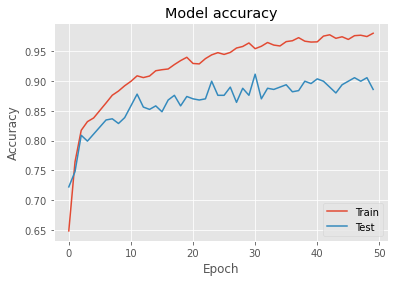
\includegraphics[scale=1]{images/fig-25.png}
\caption{VGG-16 Model Train and Test Accuracy}
\label{fig:x VGG-16 Model Train and Test Accuracy}
\end{figure}

\vspace{5mm}
\begin{figure}[hbt!]
\centering
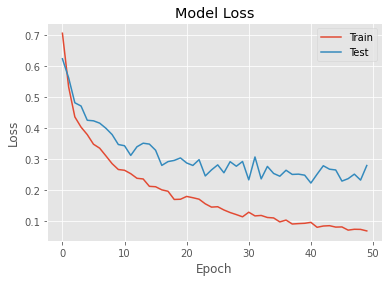
\includegraphics[scale=1]{images/fig-26.png}
\caption{VGG-16 Model Train and Test Loss}
\label{fig:x VGG-16 Model Train and Test Loss}
\end{figure}

\newpage
\noindent Model Accuracy and Loss of VGG-19 -

\vspace{5mm}
\begin{figure}[hbt!]
\centering
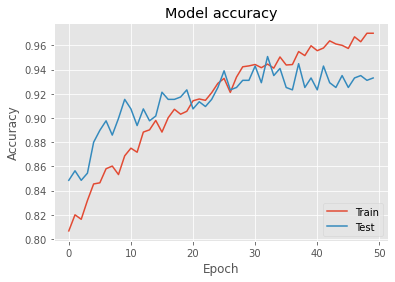
\includegraphics[scale=1]{images/fig-27.png}
\caption{VGG-19 Model Train and Test Accuracy}
\label{fig:x VGG-19 Model Train and Test Accuracy}
\end{figure}

\vspace{5mm}
\begin{figure}[hbt!]
\centering
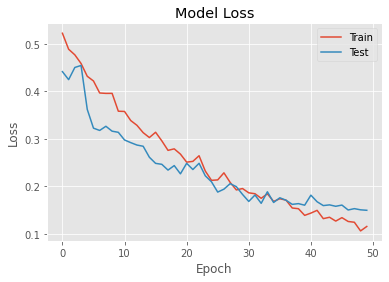
\includegraphics[scale=1]{images/fig-28.png}
\caption{VGG-19 Model Train and Test Loss}
\label{fig:x VGG-19 Model Train and Test Loss}
\end{figure}

\newpage
\vspace{5mm}
\noindent Model Accuracy and Loss of ResNet50 -
\vspace{5mm}
\begin{figure}[hbt!]
\centering
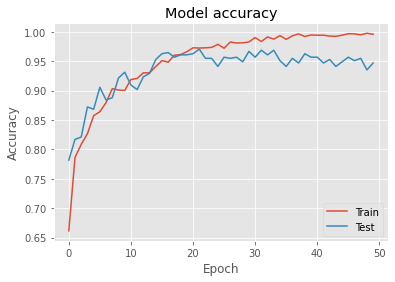
\includegraphics[scale=1]{images/fig-29.png}
\caption{ResNet50 Model Train and Test Accuracy}
\label{fig:x ResNet50 Model Train and Test Accuracy}
\end{figure}

\vspace{5mm}
\begin{figure}[hbt!]
\centering
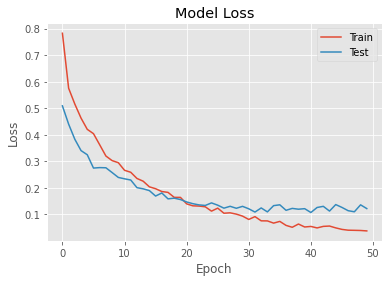
\includegraphics[scale=1]{images/fig-30.png}
\caption{ResNet50 Model Train and Test Loss}
\label{fig:x ResNet50 Model Train and Test Loss}
\end{figure}

\newpage
\vspace{5mm}
\noindent Model Accuracy and Loss of DenseNet121 -
\vspace{5mm}
\begin{figure}[hbt!]
\centering
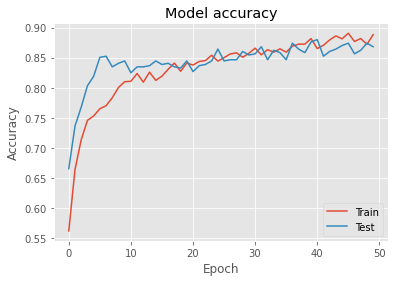
\includegraphics[scale=1]{images/fig-31.png}
\caption{DenseNet121 Model Train and Test Accuracy}
\label{fig:x DenseNet121 Model Train and Test Accuracy}
\end{figure}

\vspace{5mm}
\begin{figure}[hbt!]
\centering
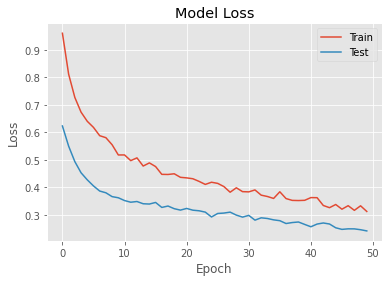
\includegraphics[scale=1]{images/fig-32.png}
\caption{DenseNet121 Model Train and Test Loss}
\label{fig:x DenseNet121 Model Train and Test Loss}
\end{figure}

\newpage
\vspace{5mm}
\noindent Model Accuracy and Loss of InceptionV3 -
\vspace{5mm}
\begin{figure}[hbt!]
\centering
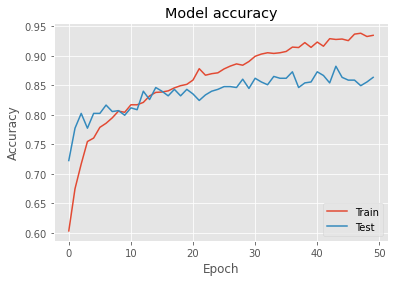
\includegraphics[scale=1]{images/fig-33.png}
\caption{InceptionV3 Model Train and Test Accuracy}
\label{fig:x InceptionV3 Model Train and Test Accuracy}
\end{figure}

\vspace{5mm}
\begin{figure}[hbt!]
\centering
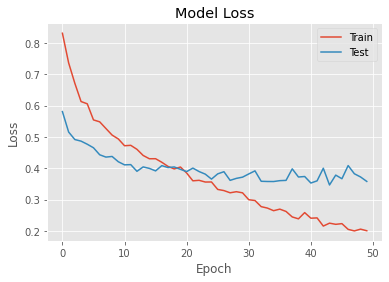
\includegraphics[scale=1]{images/fig-34.png}
\caption{InceptionV3 Model Train and Test Loss}
\label{fig:x InceptionV3 Model Train and Test Loss}
\end{figure}

\noindent The form and behavior of a learning curve may be used to analyze a machine learning model's performance, also advise what sort of config modifications should be required to enhance the production.

\vspace{5mm}
\noindent In learning curves, there are three main dynamics that you'll see. They are as follows:


\begin{itemize}
    \item Underfit
    \item Overfit
    \item Good Fit
\end{itemize}

\noindent We know that smaller relative scores on the y-axis indicate more or better learning. 

\vspace{5mm}
\begin{figure}[hbt!]
\centering
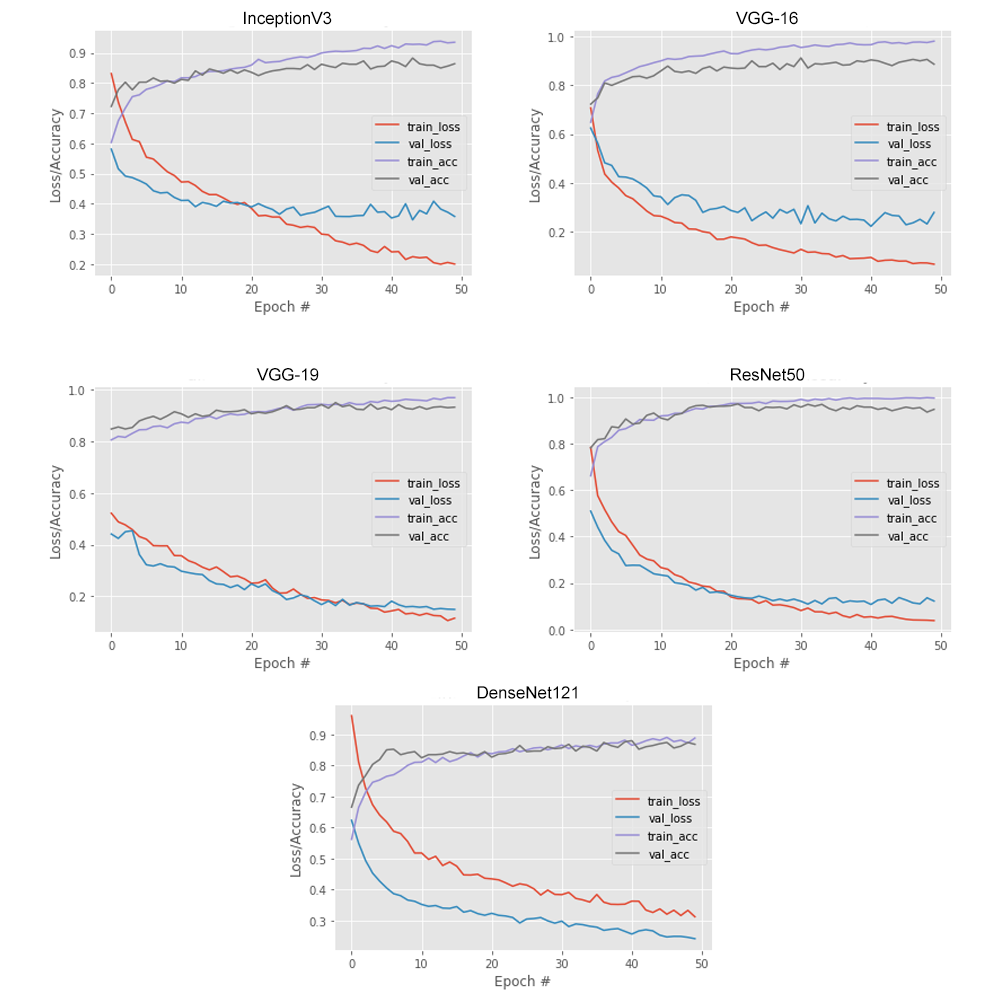
\includegraphics[scale=0.75]{images/fig-35.png}
\caption{All Model’s Train Test Accuracy and Loss Curve}
\label{fig:x All Model’s Train Test Accuracy and Loss Curve}
\end{figure}

\vspace{5mm}
\noindent Comparing All models' Accuracy and Loss graph together, we can see that VGG-19 and ResNet50 were the Good-Fit than the other models.

\vspace{5mm}
\noindent These are the Train sets, True and Predicted scores of classified and misclassified glaucoma and non-glaucoma results for each model based on the model’s train datasets prediction labels and the actual train labels. We have added a threshold of 0.5 for this train predicted visualization.

\vspace{5mm}
\noindent (the percentages are meaning the predicted train accuracy for the predicted labels calculated with the actual train labels)

\vspace{5mm}
\begin{figure}[hbt!]
\centering
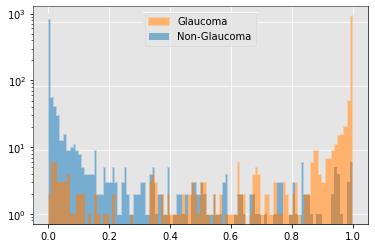
\includegraphics[scale=0.75]{images/fig-36.png}
\caption{True and Predicted Train scores of DenseNet121}
\label{fig:x True and Predicted Train scores of DenseNet121}
\end{figure}

% \centering
\begin{center}
All  151 misclassified samples (93.83\%) 

Glaucoma  74 misclassified samples (93.95\%)

Non-Glaucoma  77 misclassified samples (93.71\%)
\end{center}
\vspace{5mm}
\begin{figure}[hbt!]
\centering
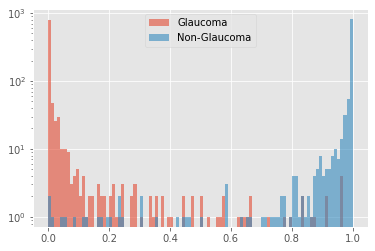
\includegraphics[scale=0.75]{images/fig-37.png}
\caption{True and Predicted Train scores of InceptionV3}
\label{fig:x True and Predicted Train scores of InceptionV3}
\end{figure}

% \centering
\begin{center}
All   48 misclassified samples (97.65\%)

Glaucoma  22 misclassified samples (97.84\%)

Non-Glaucoma  26 misclassified samples (97.45\%)
\end{center}
\vspace{5mm}
\begin{figure}[hbt!]
\centering
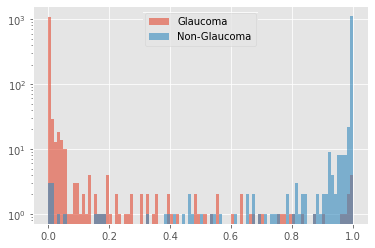
\includegraphics[scale=0.75]{images/fig-38.png}
\caption{True and Predicted Train scores of VGG-16}
\label{fig:x True and Predicted Train scores of VGG-16}
\end{figure}

\newpage
% \centering
\begin{center}
All   47 misclassified samples (98.08\%)

Glaucoma  20 misclassified samples (98.37\%)

Non-Glaucoma  27 misclassified samples (97.79\%)
\end{center}
\vspace{5mm}
\begin{figure}[hbt!]
\centering
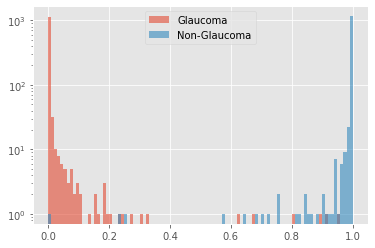
\includegraphics[scale=0.75]{images/fig-39.png}
\caption{True and Predicted Train scores of VGG-19}
\label{fig:x True and Predicted Train scores of VGG-19}
\end{figure}
\begin{center}
All   17 misclassified samples (99.31\%)

Glaucoma  14 misclassified samples (98.86\%)

Non-Glaucoma   3 misclassified samples (99.75\%)
\end{center}
\vspace{5mm}
\begin{figure}[hbt!]
\centering
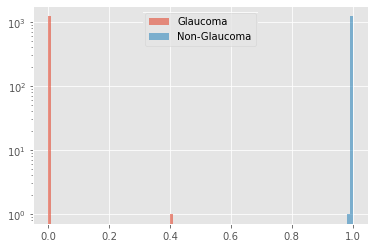
\includegraphics[scale=0.75]{images/fig-40.png}
\caption{True and Predicted Train scores of ResNet50}
\label{fig:x True and Predicted Train scores of ResNet50}
\end{figure}

\newpage
\begin{center}
All    0 misclassified samples (100.00\%)

Glaucoma   0 misclassified samples (100.00\%)

Non-Glaucoma   0 misclassified samples (100.00\%)
\end{center}
\vspace{5mm}
Now, We have called the same function that we have used for the above Train predicted labels again with the same threshold of 0.5. But for now we have used the validation datasets prediction labels. And the results were - 

\noindent \textit{(the percentages are meaning the predicted test/validation accuracy for the predicted labels calculated with the actual test/validation labels)}

\noindent \textit{( Here, G = Glaucoma and n-G = Non-Glaucoma )}

\begin{center}
\begin{table}[hbt!]
\centering
\begin{tabular}{|p{3cm}|p{3cm}|p{3cm}|c|}
\hline
% \parbox{\centering \textbf{Model}} & \parbox{\centering \textbf{All misclassified}} & \parbox{\centering \textbf{G misclassified}} & \parbox{\centering \textbf{n-G misclassified}} \\

\centering{\textbf{Model} & \centering\textbf{All misclassified} & \centering\textbf{G misclassified} & \textbf{n-G misclassified}} \\
\hline
\centering DenseNet121 & \centering 9 (86.76\%) & \centering 4 (88.24\%) & 5 (85.29\%)\\
\hline
\centering InceptionV3 & \centering 24 (85.88\%) & \centering 16 (81.18\%) & 8 (90.59\%)\\
\hline
\centering VGG-16 & \centering 8 (88.24\%) & \centering 7 (79.41\%) & 1 (97.06\%)\\
\hline
\centering VGG-19 & \centering 4 (94.12\%) & \centering 3 (91.18\%) & 1 (97.06\%)\\
\hline
\centering ResNet50 & \centering 3 (95.59\%) & \centering 1 (97.06\%) & 2 (94.12\%)\\
\hline
\end{tabular}
\caption{True and Predicted Test scores of all Model}
\label{tab:True and Predicted Test scores of all Model}
\end{table}
\end{center}



\vspace{5mm}
\noindent Now we have taken a single predicted batch from each model’s prediction with the 0.5 threshold and plotted the misclassified glaucoma and non-glaucoma images, which we will use in Lime (XAI framework) to explain later.

\noindent \textit{( Here, G = Glaucoma and n-G = Non-Glaucoma )}
\begin{center}
\begin{table}[hbt!]
\centering
\begin{tabular}{|c | c | c| c |}
\hline
\textbf{Model} & \textbf{Batch} & \textbf{G misclassified} & \textbf{n-G misclassified}}\\

\hline
DenseNet121 & 2 (32 in each) & 3 &  5\\
\hline
InceptionV3 & 2 (32 in each) & 2 & 7\\
\hline
VGG-16 & 2 (32 in each) & 2 & 3\\
\hline
VGG-19 & 2 (32 in each) & 1 & 4\\
\hline
ResNet50 & 2 (32 in each) & 0 & 3\\
\hline

\end{tabular}
\caption{True and Predicted Test scores of all Model}
\label{tab:True and Predicted Test scores of all Model}
\end{table}
\end{center}
\newpage
\vspace{5mm}
\noindent These are some of the misclassified images for all models with and undoing the existing preprocessing. Basically the model’s preprocessing for these images ruined their actual color and contrast.  Which led the model to predict wrong. By undoing the existing preprocessing we can see that for DesneNet121 the images got a little reddish and for other models, It got bluish.

\vspace{5mm}
\begin{figure}[hbt!]
\centering
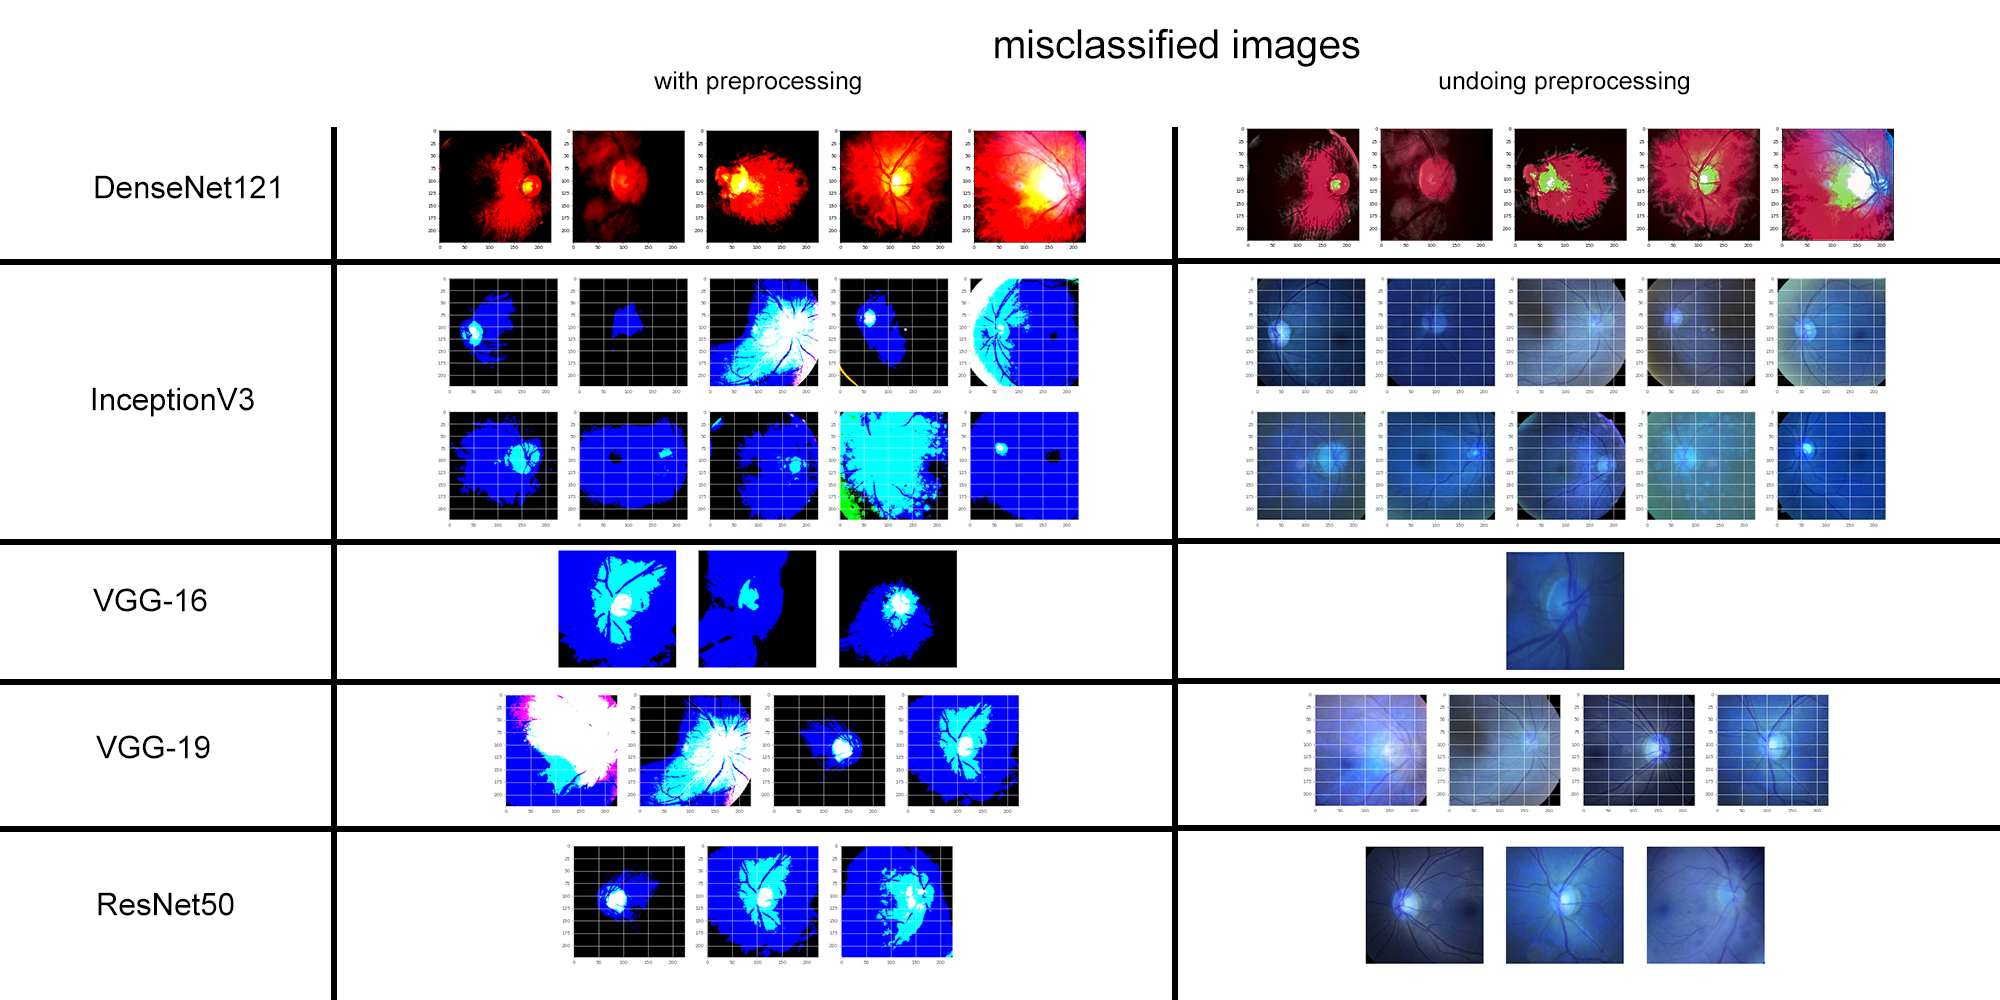
\includegraphics[scale=0.42]{images/fig-41.png}
\caption{Misclassified images for all models with and without preprocessing}
\label{fig:x True and Predicted Train scores of ResNet50}
\end{figure}

\vspace{5mm}
\noindent Now we will show the explanation for these preprocessed and misclassified images using an XAI[40] framework, \textbf{LIME}. Then we will apply Lime again on a single predicted raw fundus -image directly from the test dataset (labelled) directory to see the difference between a correctly predicted fundus image[42] and wrong predicted fundus image.
Given below are the the misclassified image with preprocessing, Superpixels focused area and the model prediction explanation by Lime in DenseNet121

\vspace{5mm}
\begin{figure}[hbt!]
\centering
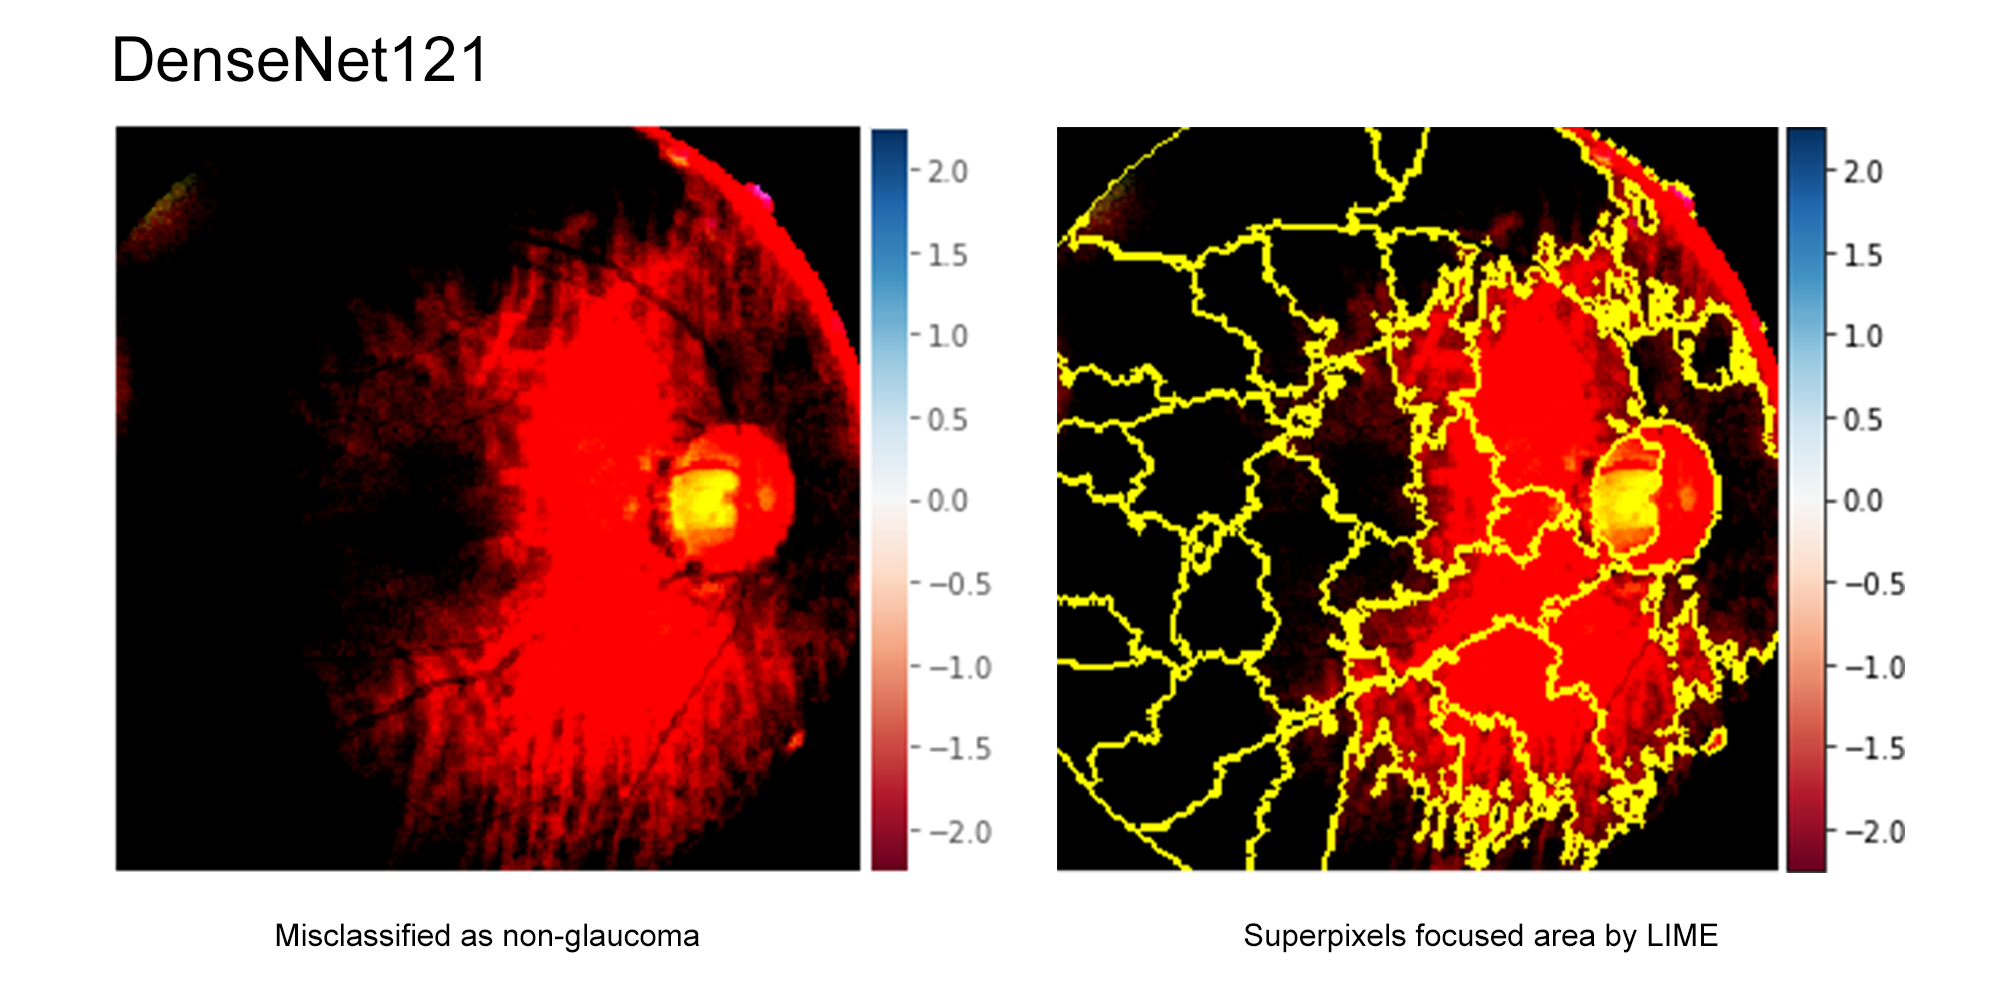
\includegraphics[scale=0.45]{images/fig-42.png}
\caption{Misclassified image with preprocessing and Superpixels focused area by Lime in DenseNet121}
\label{fig:x Misclassified image with preprocessing and Superpixels focused area by Lime in DenseNet121}
\end{figure}

\vspace{5mm}
\begin{figure}[hbt!]
\centering
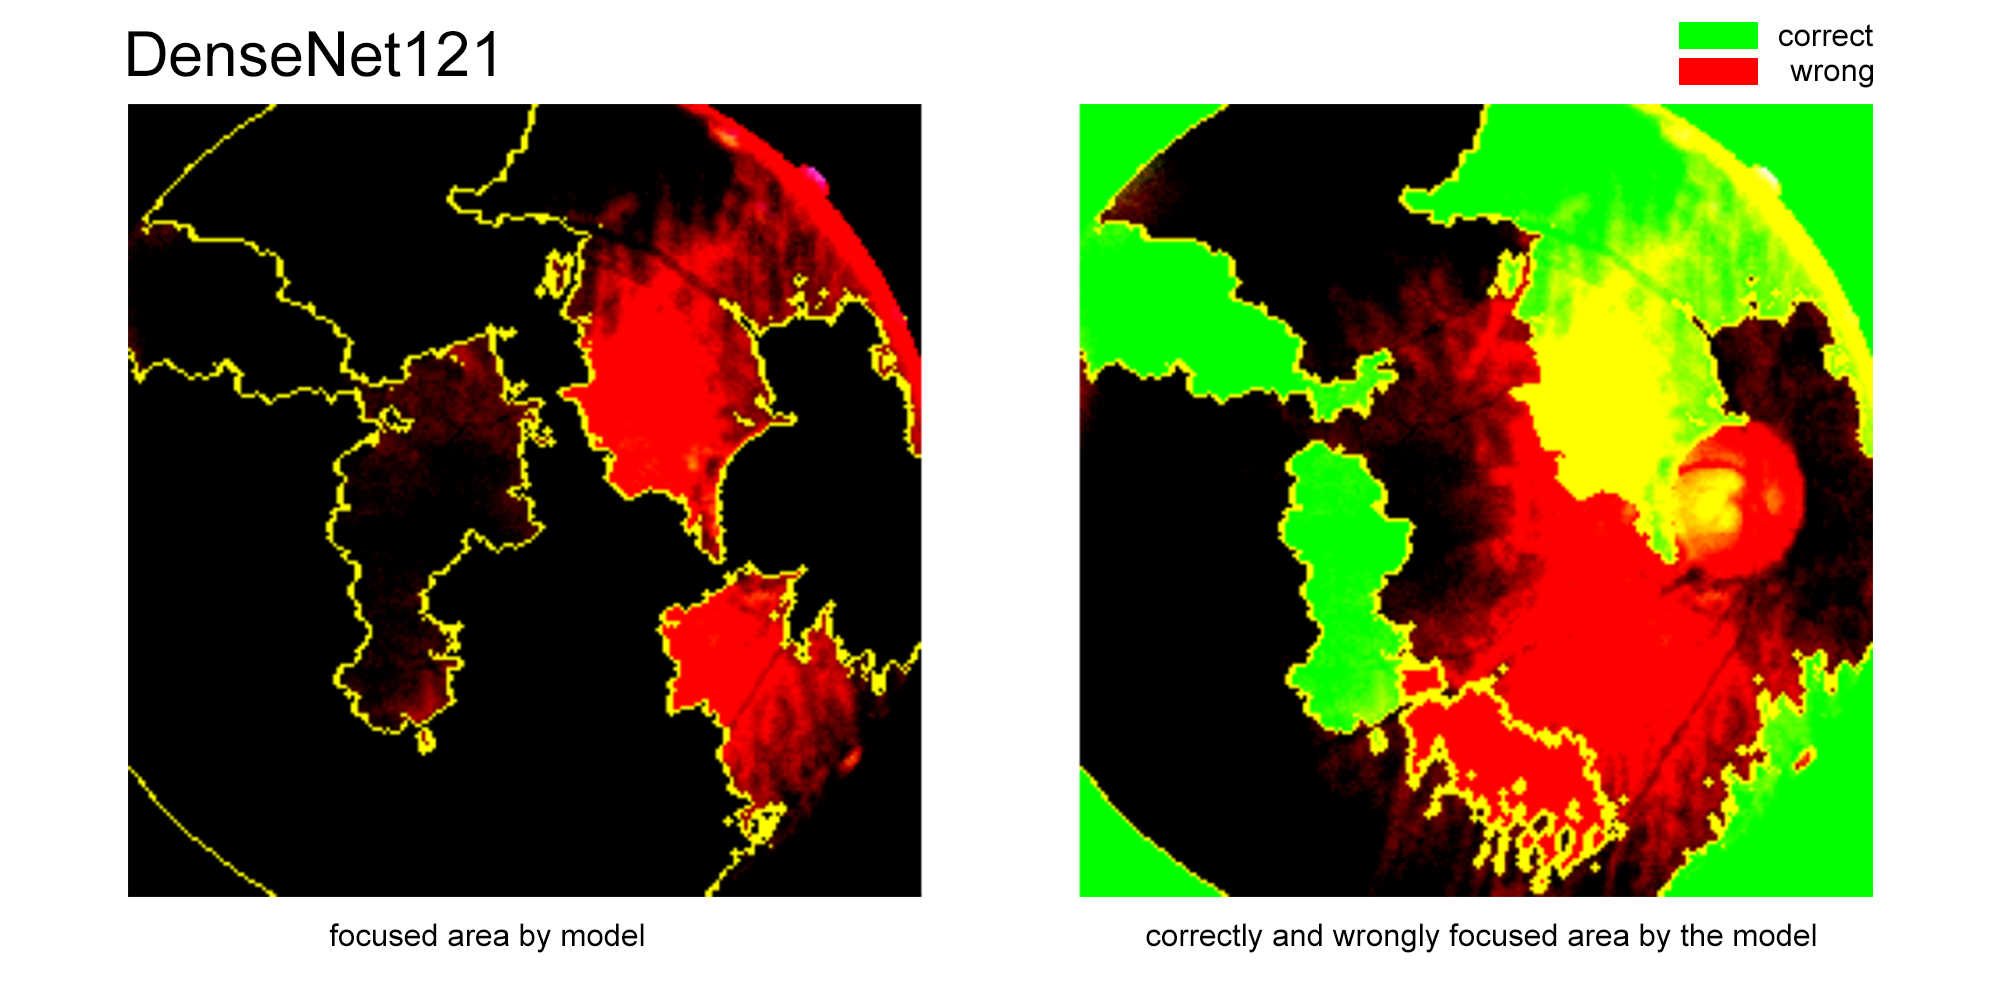
\includegraphics[scale=0.45]{images/fig-43.png}
\caption{Lime Explanation for DenseNet121}
\label{fig:x Lime Explanation for DenseNet121}
\end{figure}

\newpage
\vspace{5mm}
\noindent Given below are the the misclassified image with preprocessing, Superpixels focused area and the model prediction explanation by Lime in InceptionV3 -

\vspace{5mm}
\begin{figure}[hbt!]
\centering
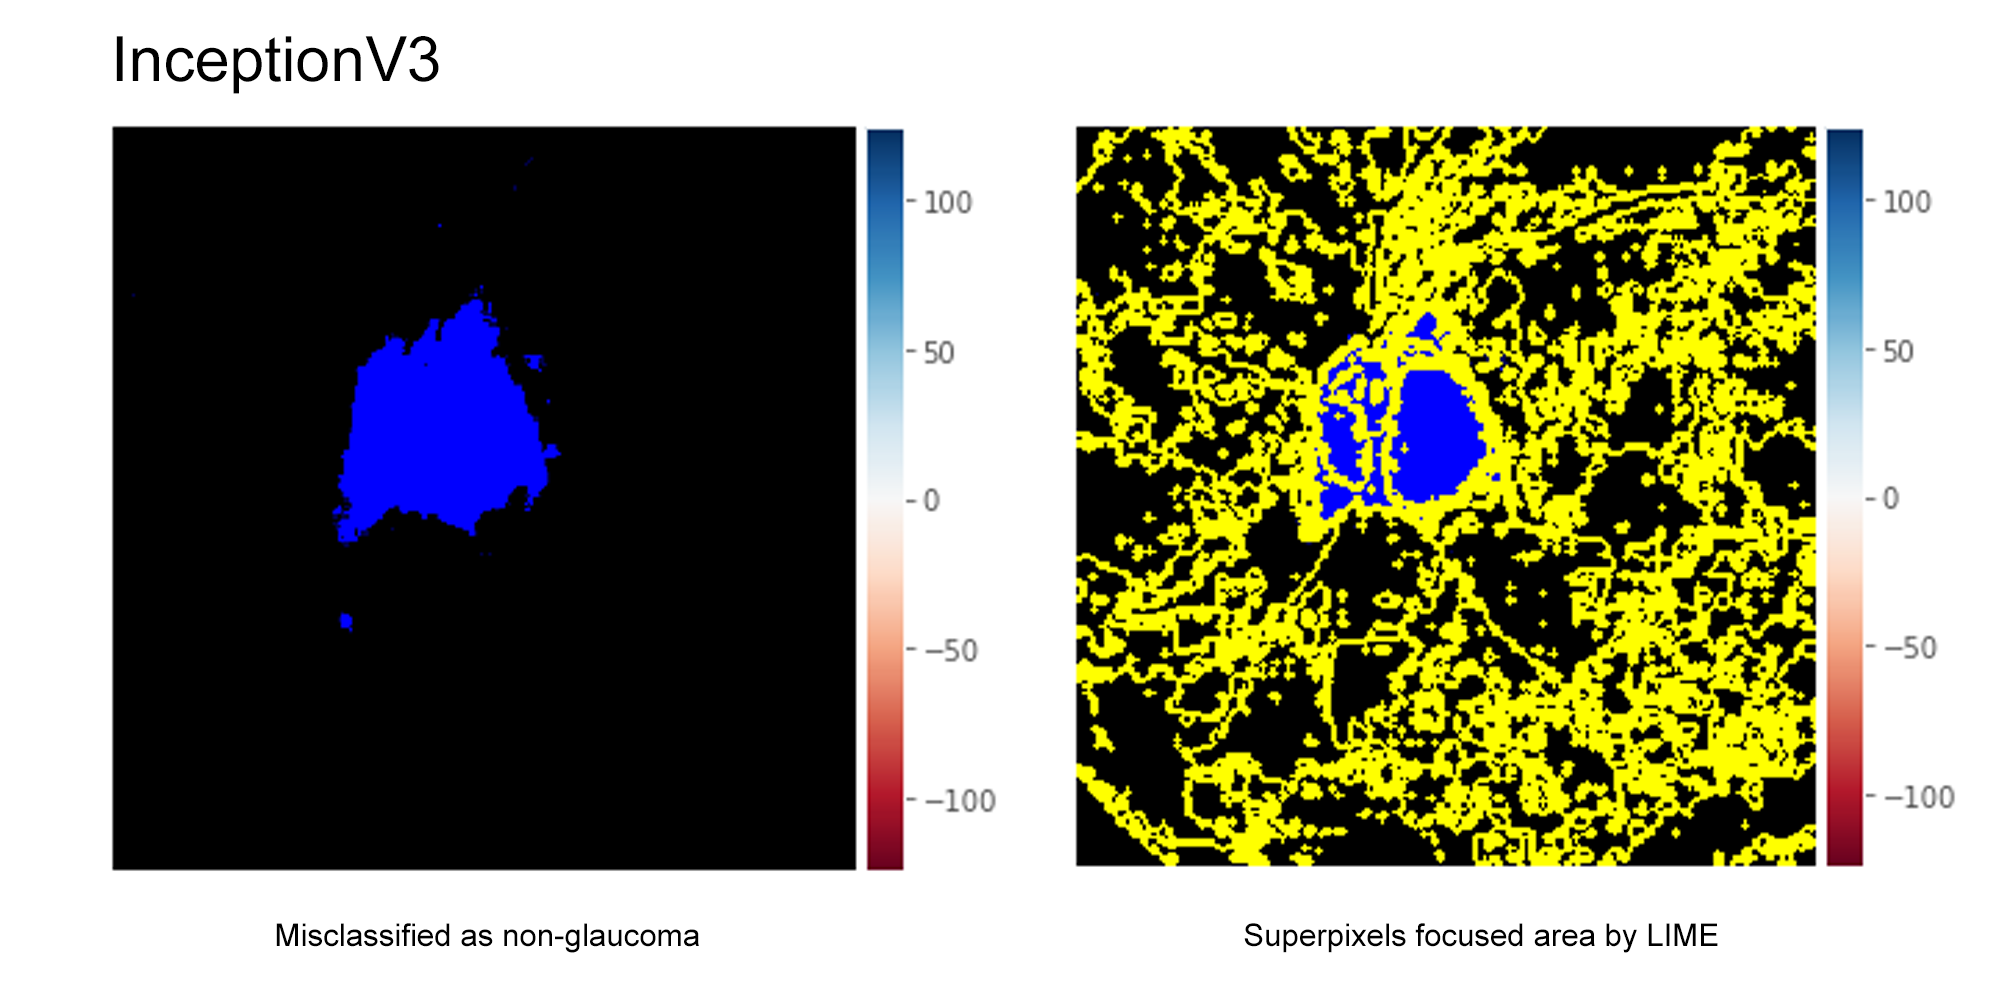
\includegraphics[scale=0.45]{images/fig-44.png}
\caption{Misclassified image with preprocessing and Superpixels focused area by Lime in InceptionV3
}
\label{fig:x Misclassified image with preprocessing and Superpixels focused area by Lime in InceptionV3
}
\end{figure}

\vspace{5mm}
\begin{figure}[hbt!]
\centering
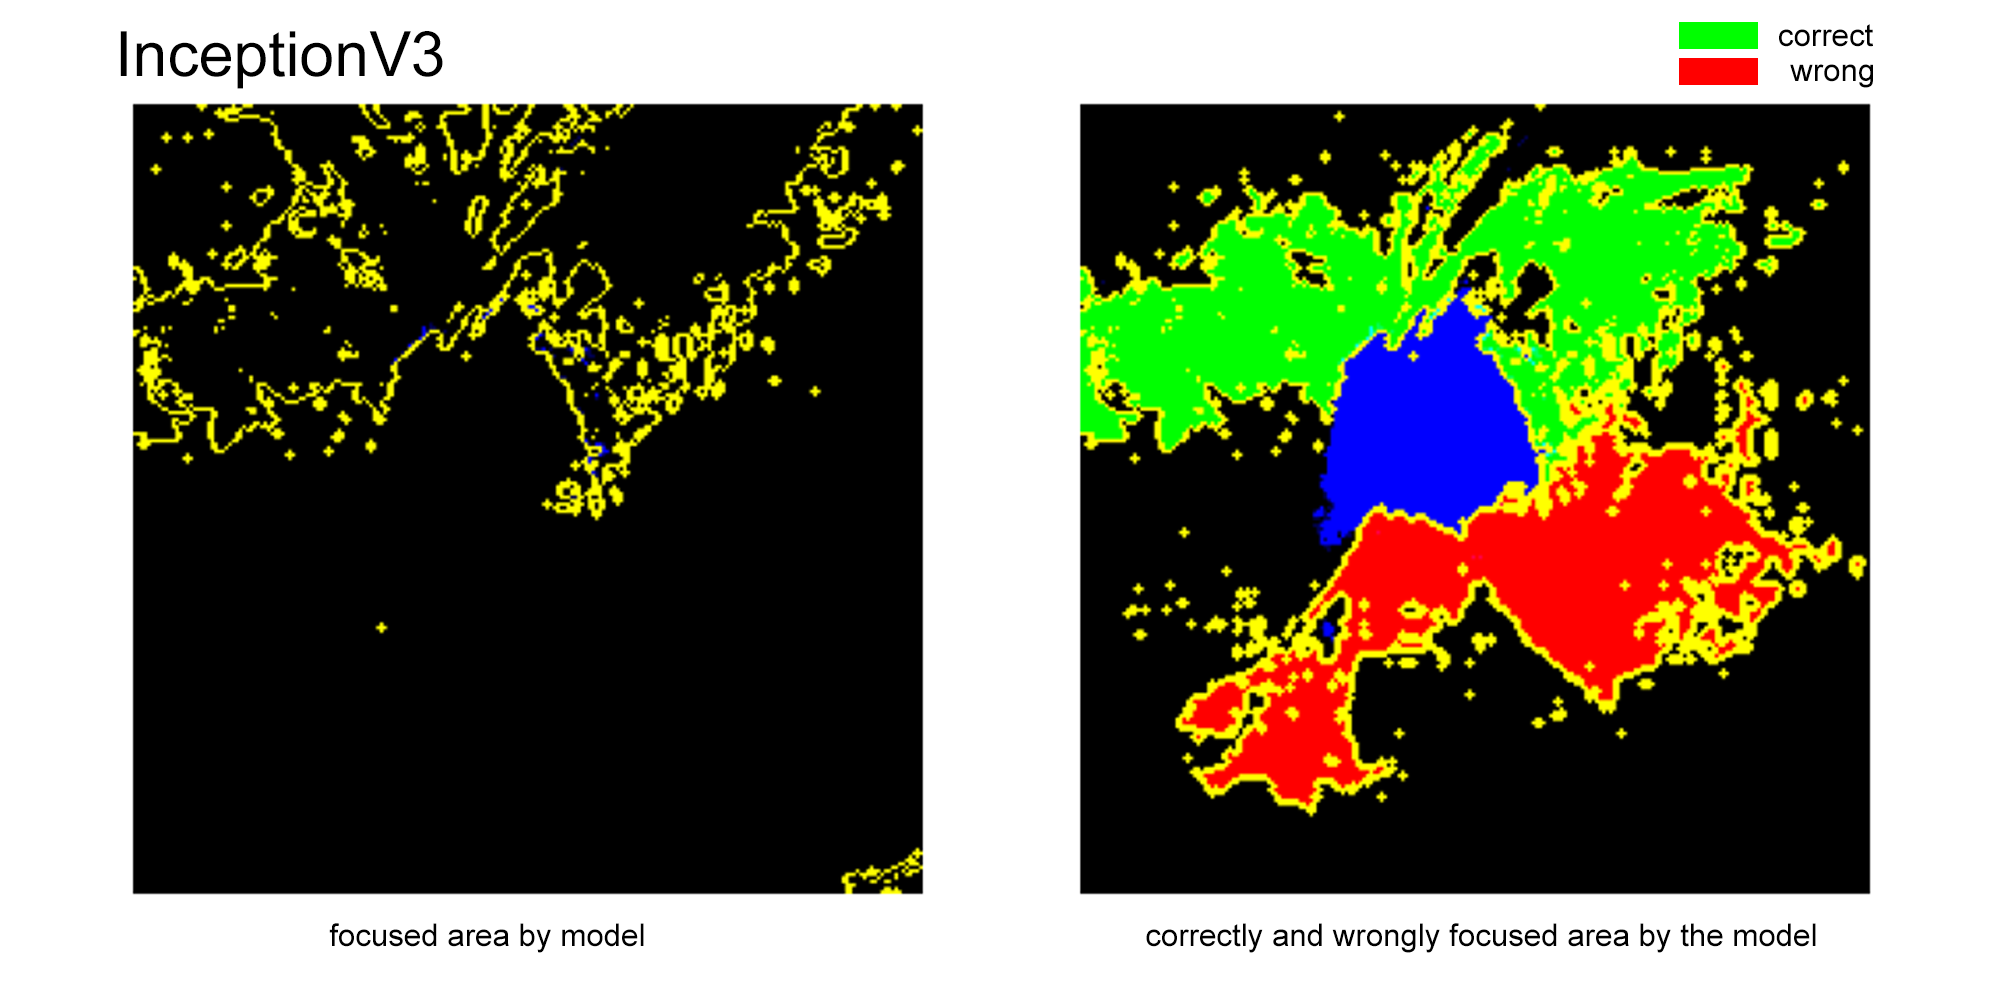
\includegraphics[scale=0.45]{images/fig-45.png}
\caption{Lime Explanation for InceptionV3}
\label{fig:x Lime Explanation for InceptionV3}
\end{figure}

\newpage
\vspace{5mm}
\noindent Given below are the the misclassified image with preprocessing, Superpixels focused area and the model prediction explanation by Lime in VGG-16 -

\vspace{5mm}
\begin{figure}[hbt!]
\centering
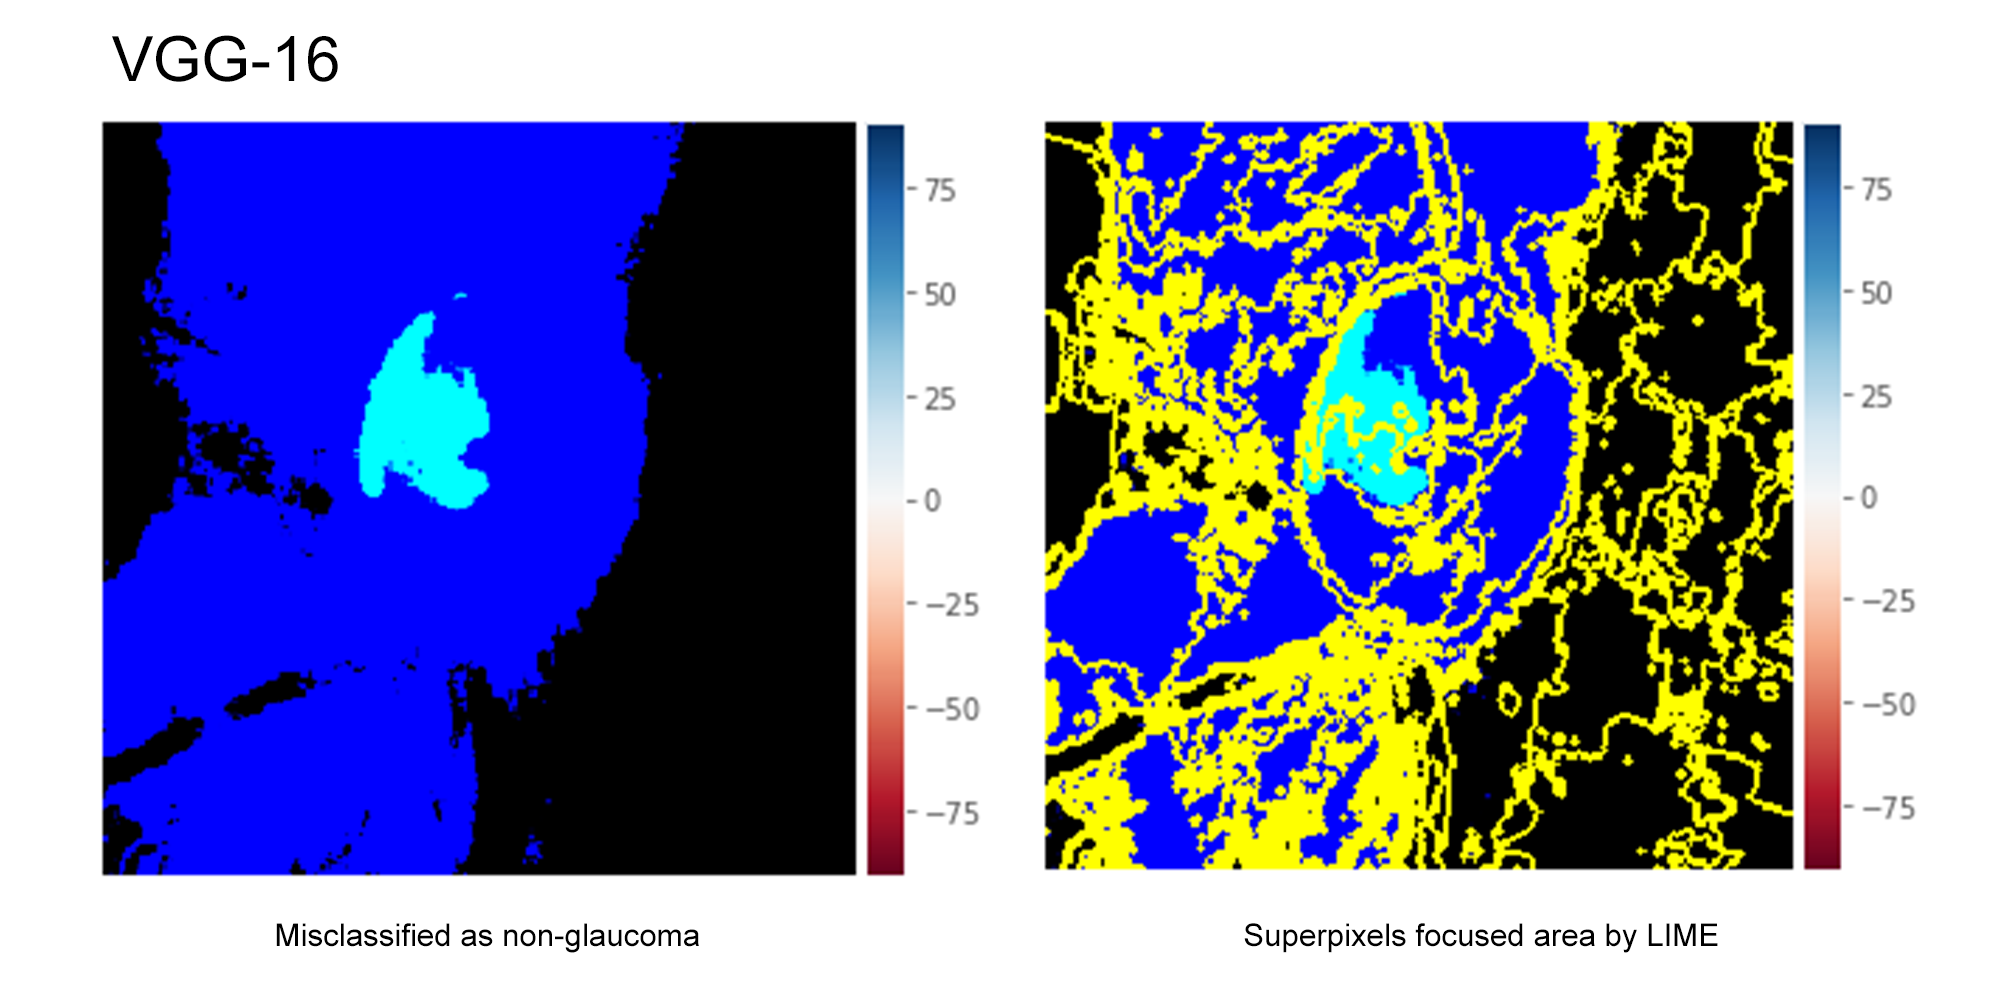
\includegraphics[scale=0.45]{images/fig-46.png}
\caption{Misclassified image with preprocessing and Superpixels focused area by Lime in VGG-16}
\label{fig:x Misclassified image with preprocessing and Superpixels focused area by Lime in VGG-16}
\end{figure}

\vspace{5mm}
\begin{figure}[hbt!]
\centering
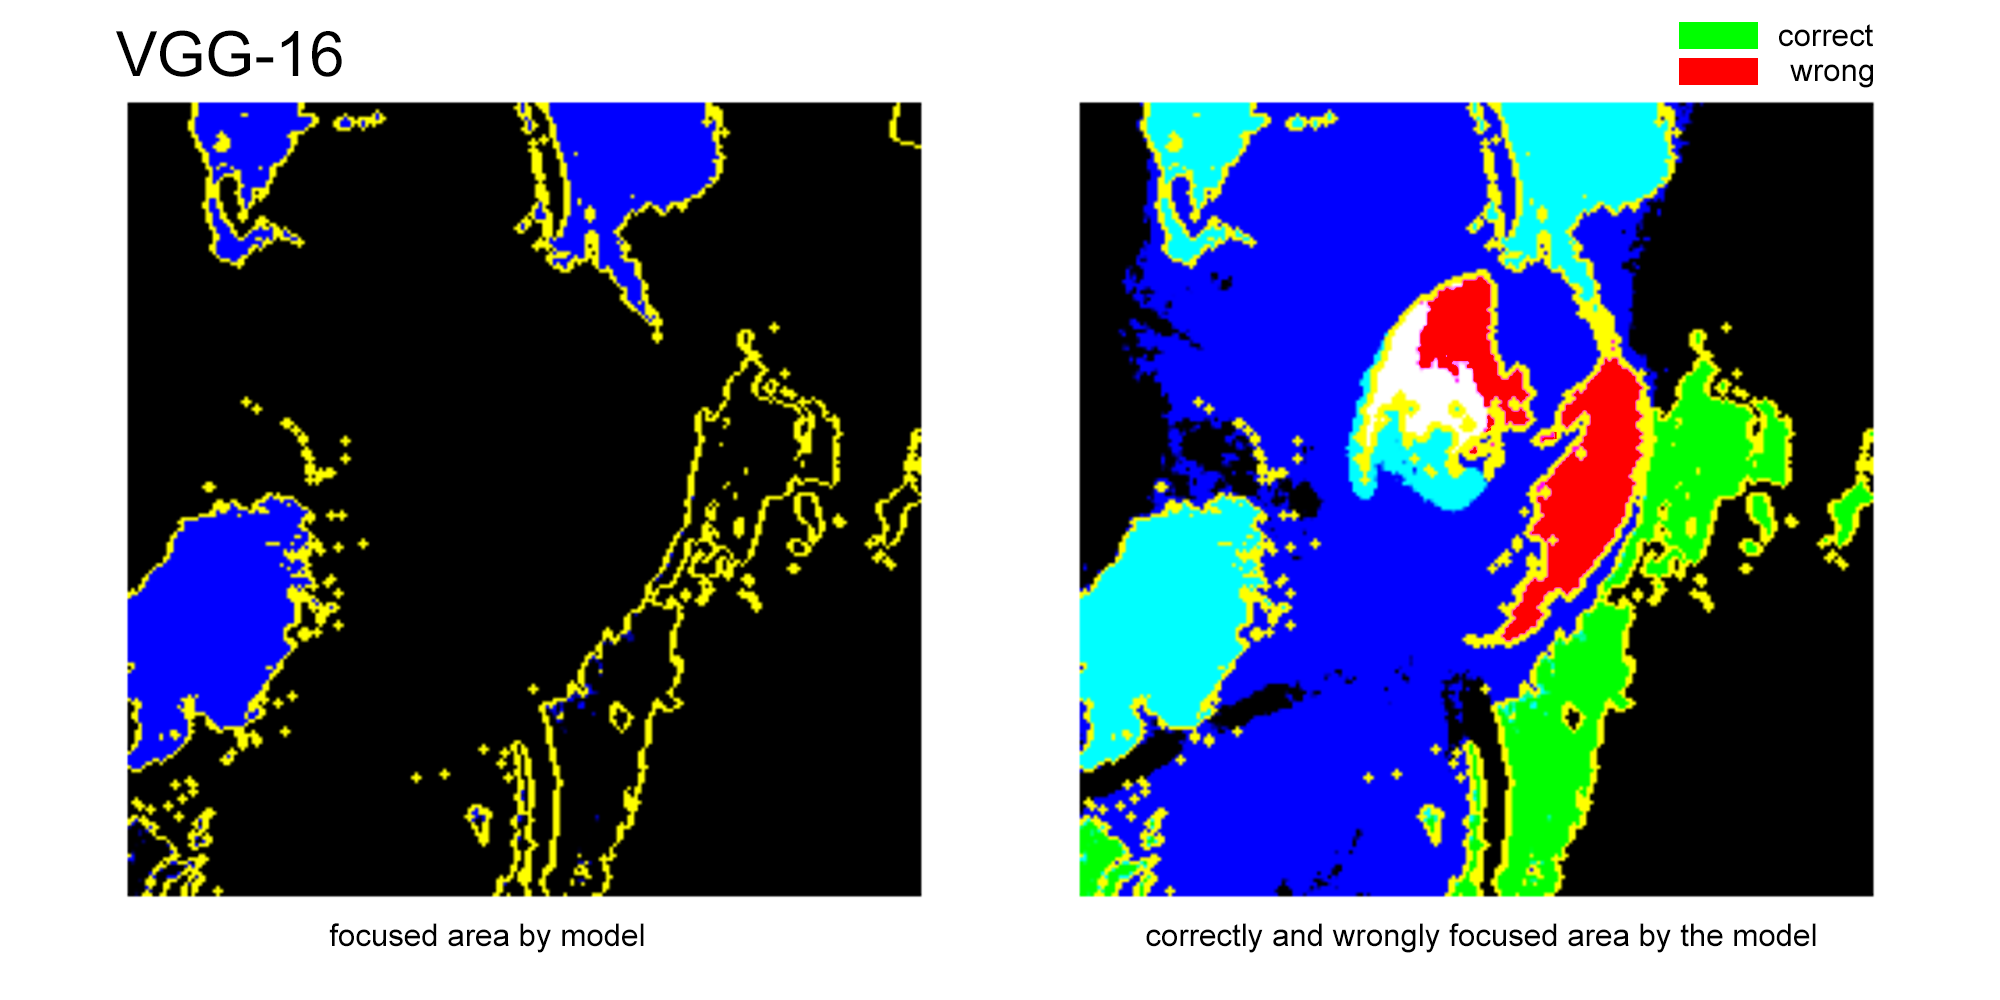
\includegraphics[scale=0.45]{images/fig-47.png}
\caption{Lime Explanation for VGG-16}
\label{fig:x Lime Explanation for VGG-16}
\end{figure}

\newpage
\vspace{5mm}
\noindent Given below are the the misclassified image with preprocessing, Superpixels focused area and the model prediction explanation by Lime in VGG-19 -

\vspace{5mm}
\begin{figure}[hbt!]
\centering
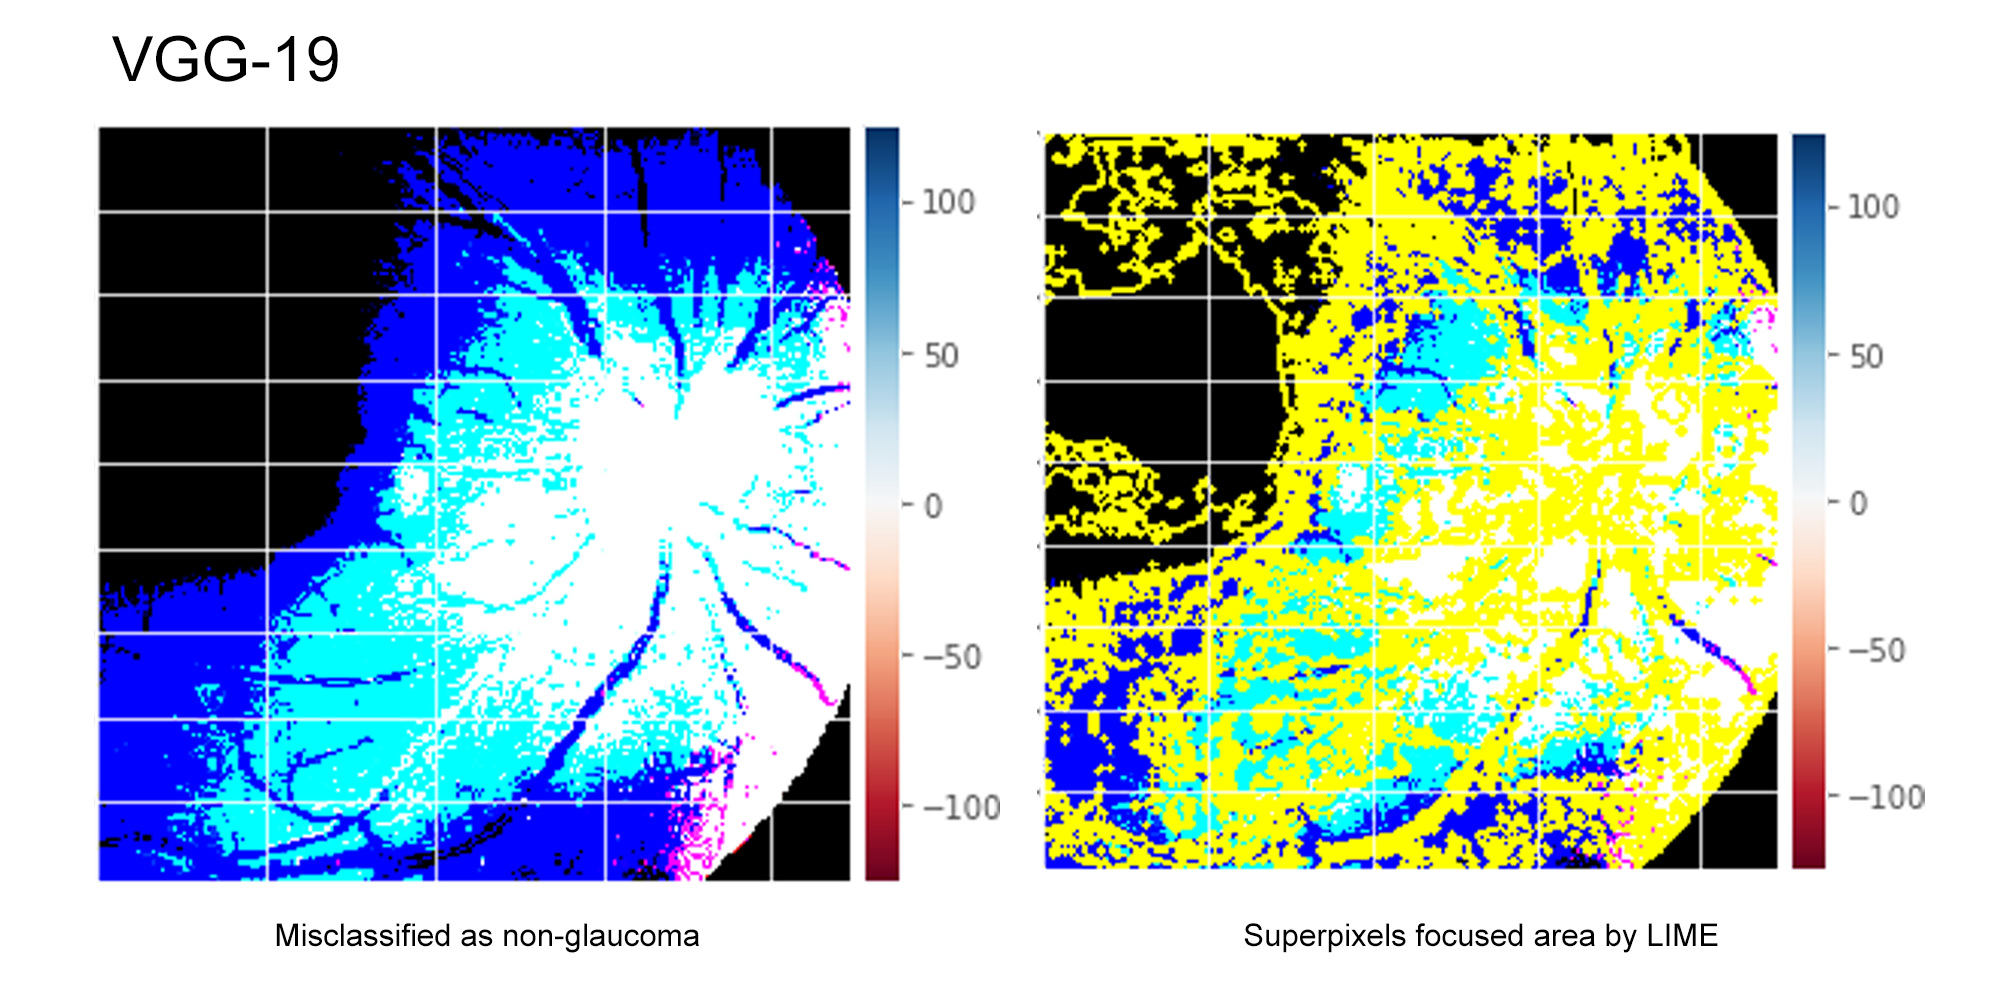
\includegraphics[scale=0.45]{images/fig-48.png}
\caption{Misclassified image with preprocessing and Superpixels focused area by Lime in VGG-19}
\label{fig:x Misclassified image with preprocessing and Superpixels focused area by Lime in VGG-19}
\end{figure}

\vspace{5mm}
\begin{figure}[hbt!]
\centering
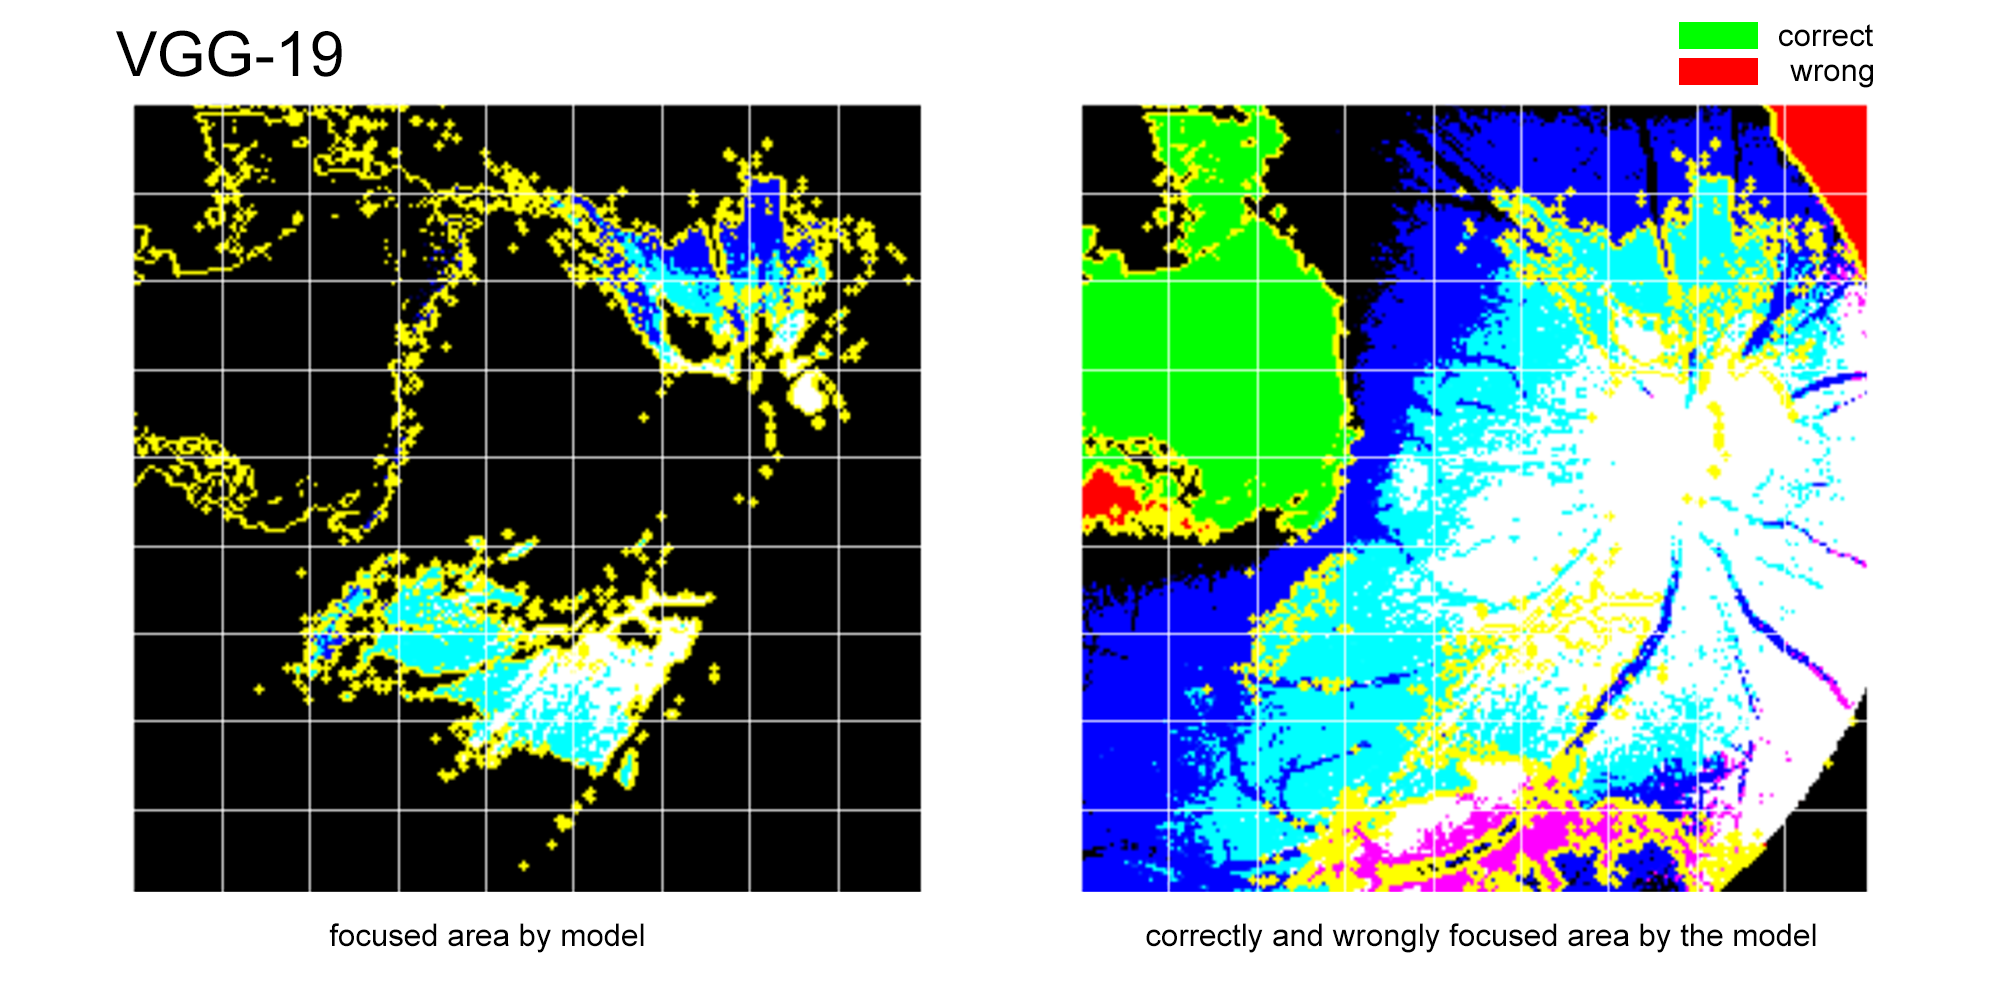
\includegraphics[scale=0.45]{images/fig-49.png}
\caption{Lime Explanation for VGG-19}
\label{fig:x Lime Explanation for VGG-19}
\end{figure}

\newpage
\vspace{5mm}
\noindent Given below are the the misclassified image with preprocessing, Superpixels focused area and the model prediction explanation by Lime in ResNet50 -

\vspace{5mm}
\begin{figure}[hbt!]
\centering
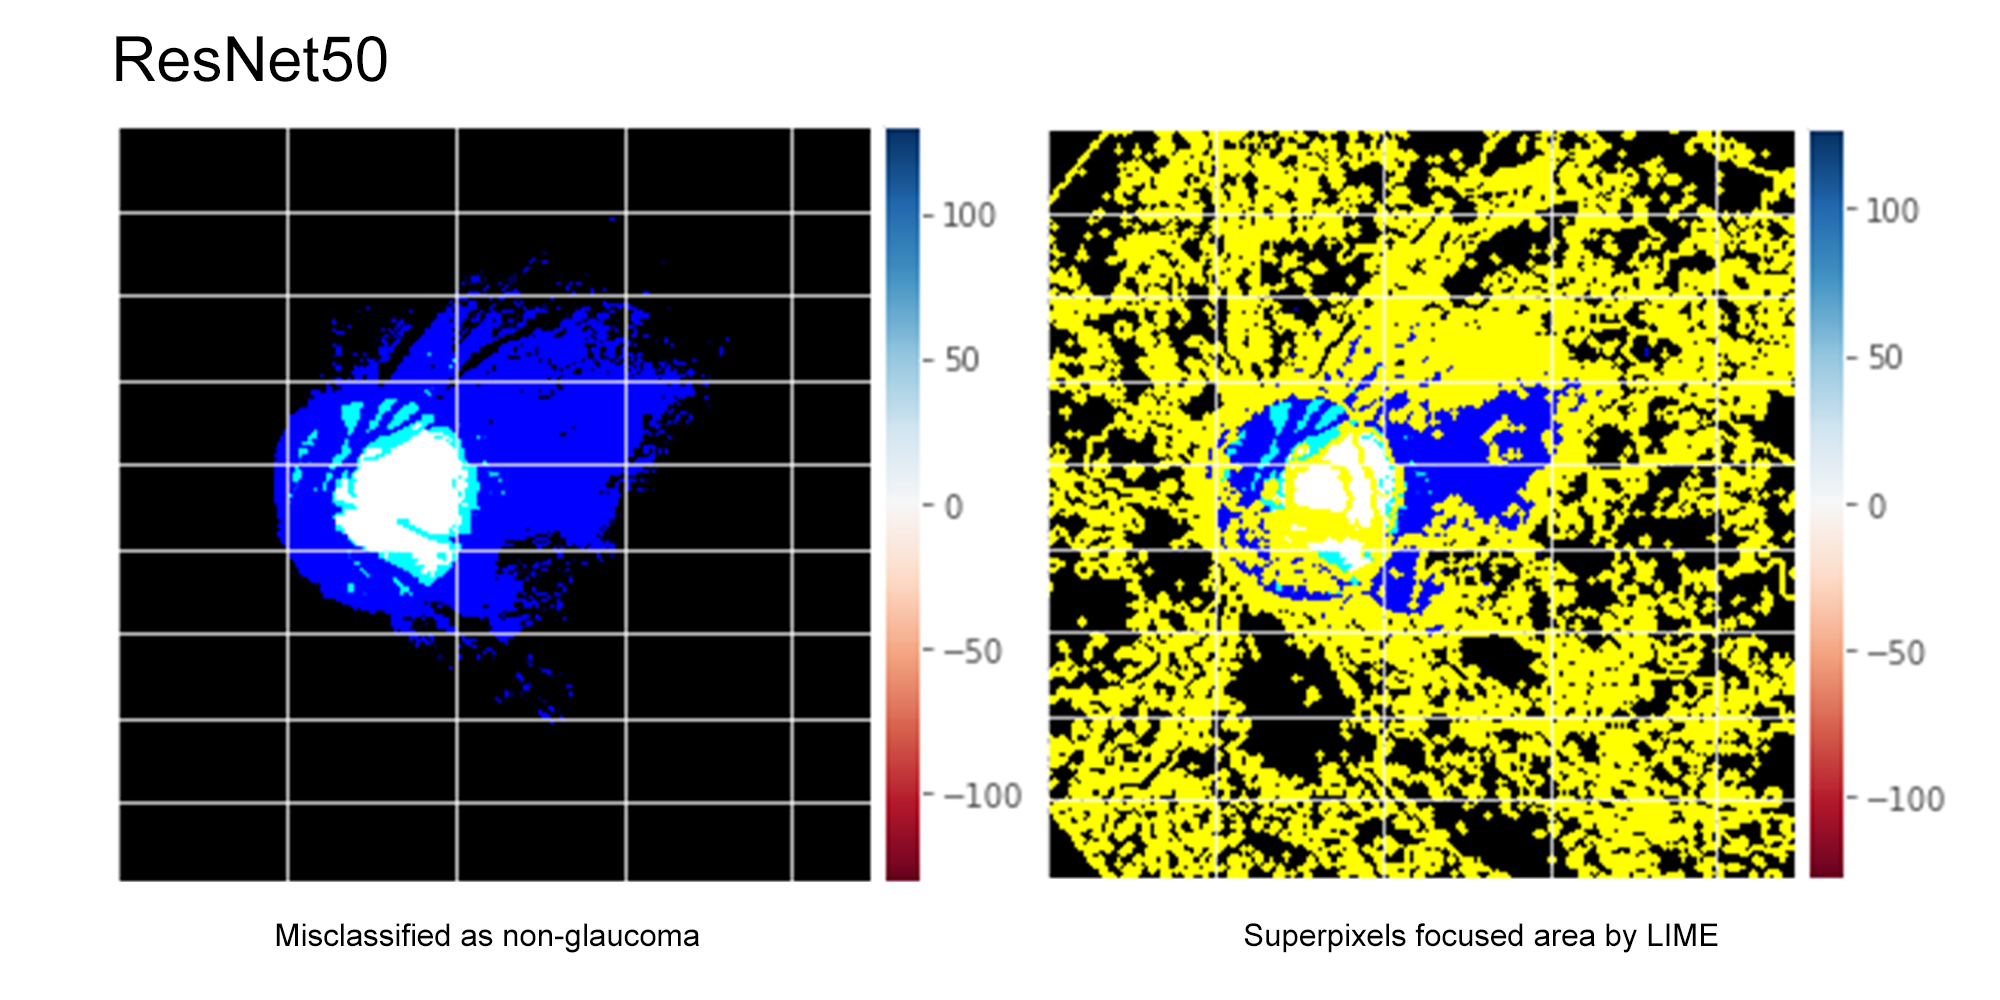
\includegraphics[scale=0.45]{images/fig-50.png}
\caption{Misclassified image with preprocessing and Superpixels focused area by Lime in ResNet50}
\label{fig:x Misclassified image with preprocessing and Superpixels focused area by Lime in ResNet50}
\end{figure}

\vspace{5mm}
\begin{figure}[hbt!]
\centering
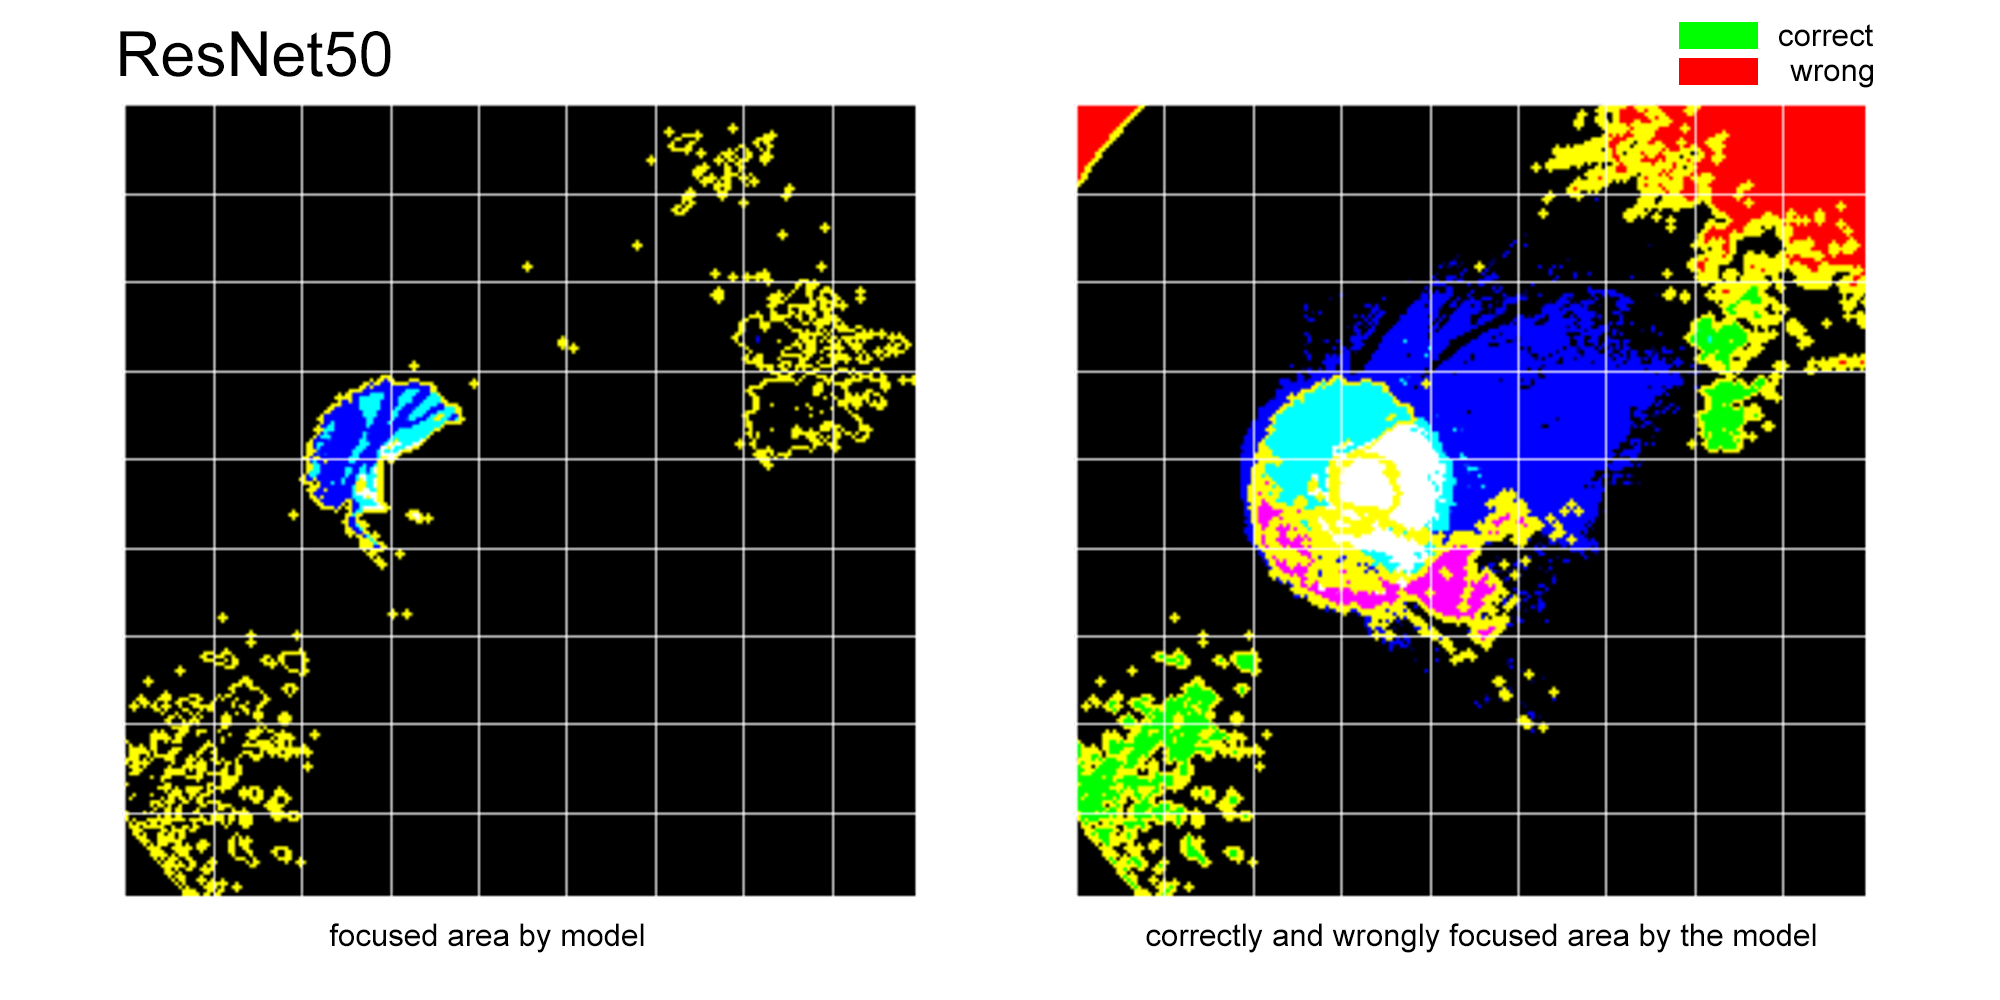
\includegraphics[scale=0.45]{images/fig-51.png}
\caption{Lime Explanation for ResNet50}
\label{fig:x Lime Explanation for ResNet50}
\end{figure}

\newpage
\vspace{5mm}
Now for the single predicted raw fundus image -

\vspace{5mm}
\begin{figure}[hbt!]
\centering
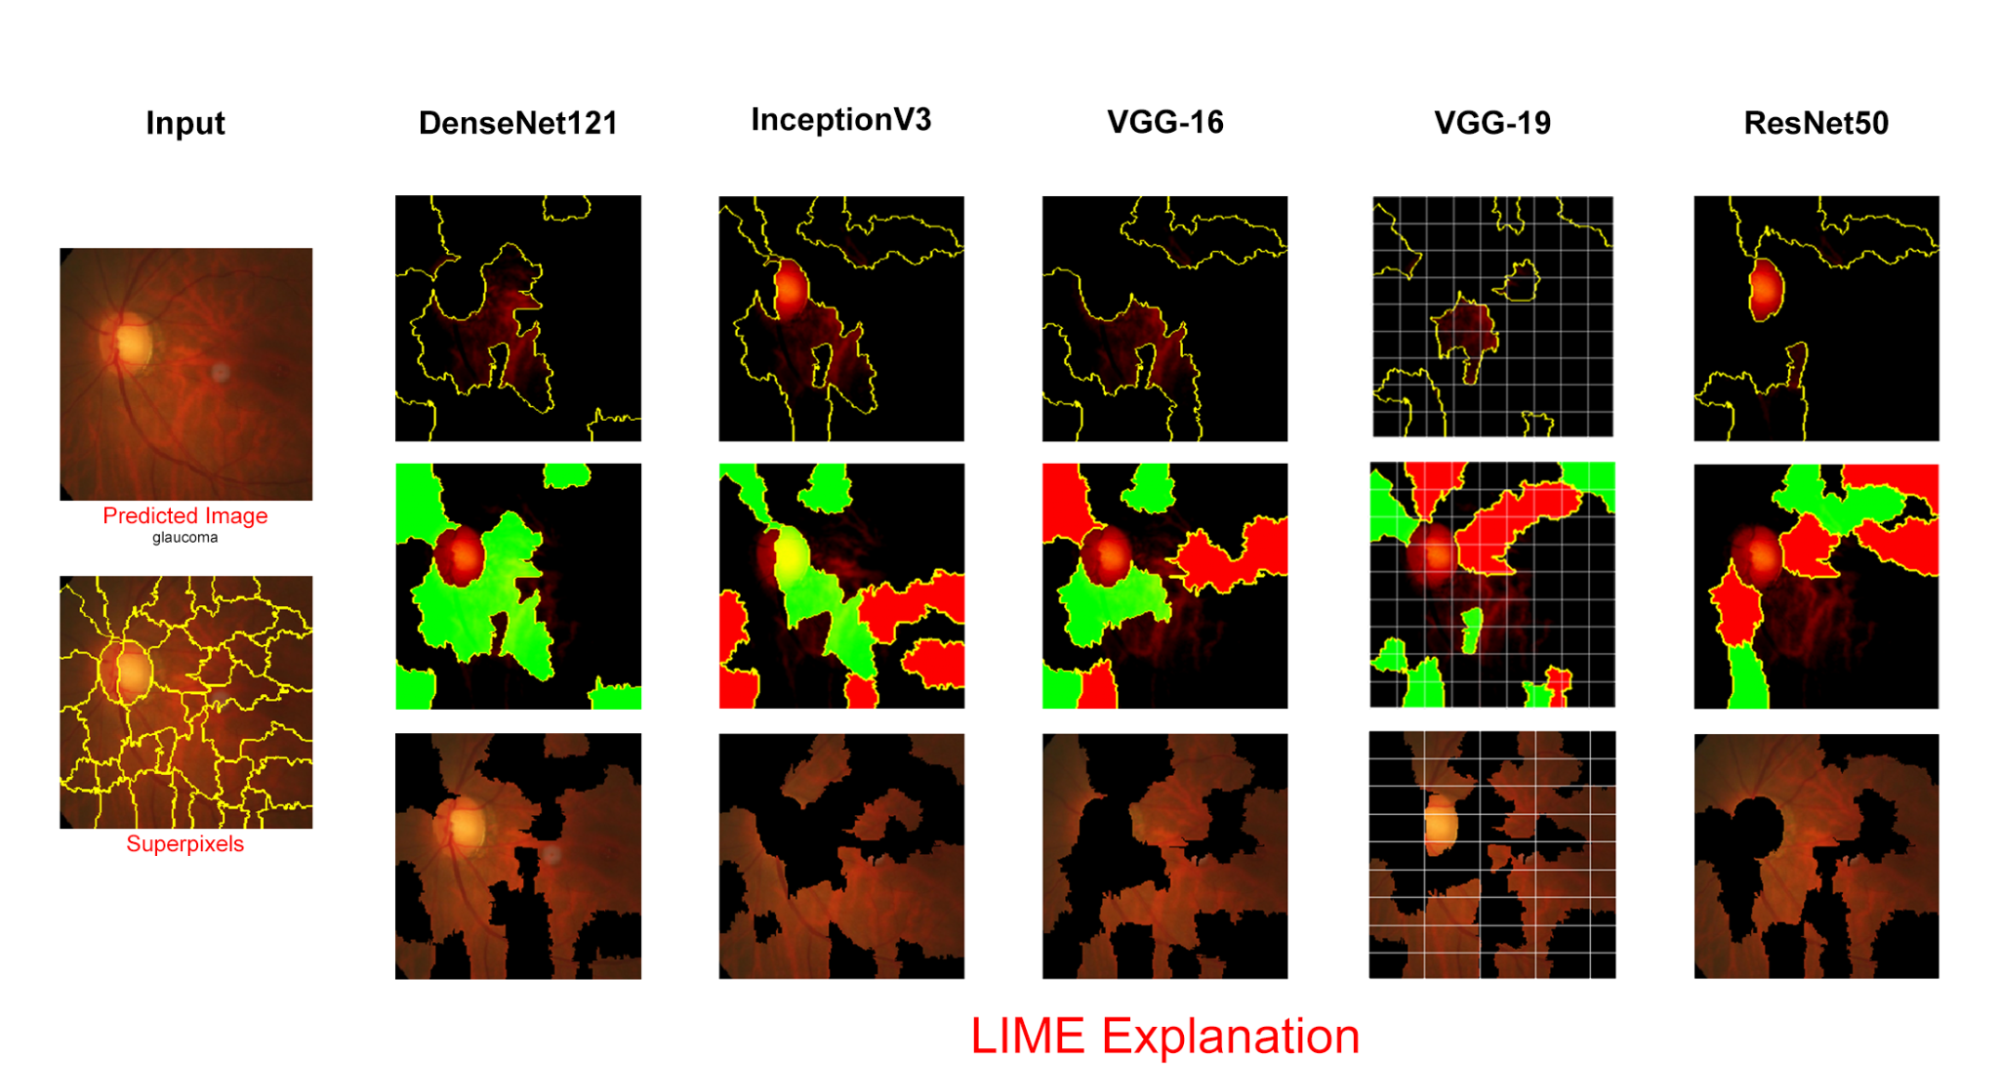
\includegraphics[scale=0.20]{images/fig-52.png}
\caption{Lime Explanation for all models single image predictions}
\label{fig:x Lime Explanation for all models single image predictions}
\end{figure}

\newpage
\section{Result}
These are the single image predictions of all models - 

\noindent\textit{( here outputs are given in [n,m] format, where “m” means glaucoma score and “n” means non-glaucoma score )}

\vspace{5mm}
\begin{figure}[hbt!]
\centering
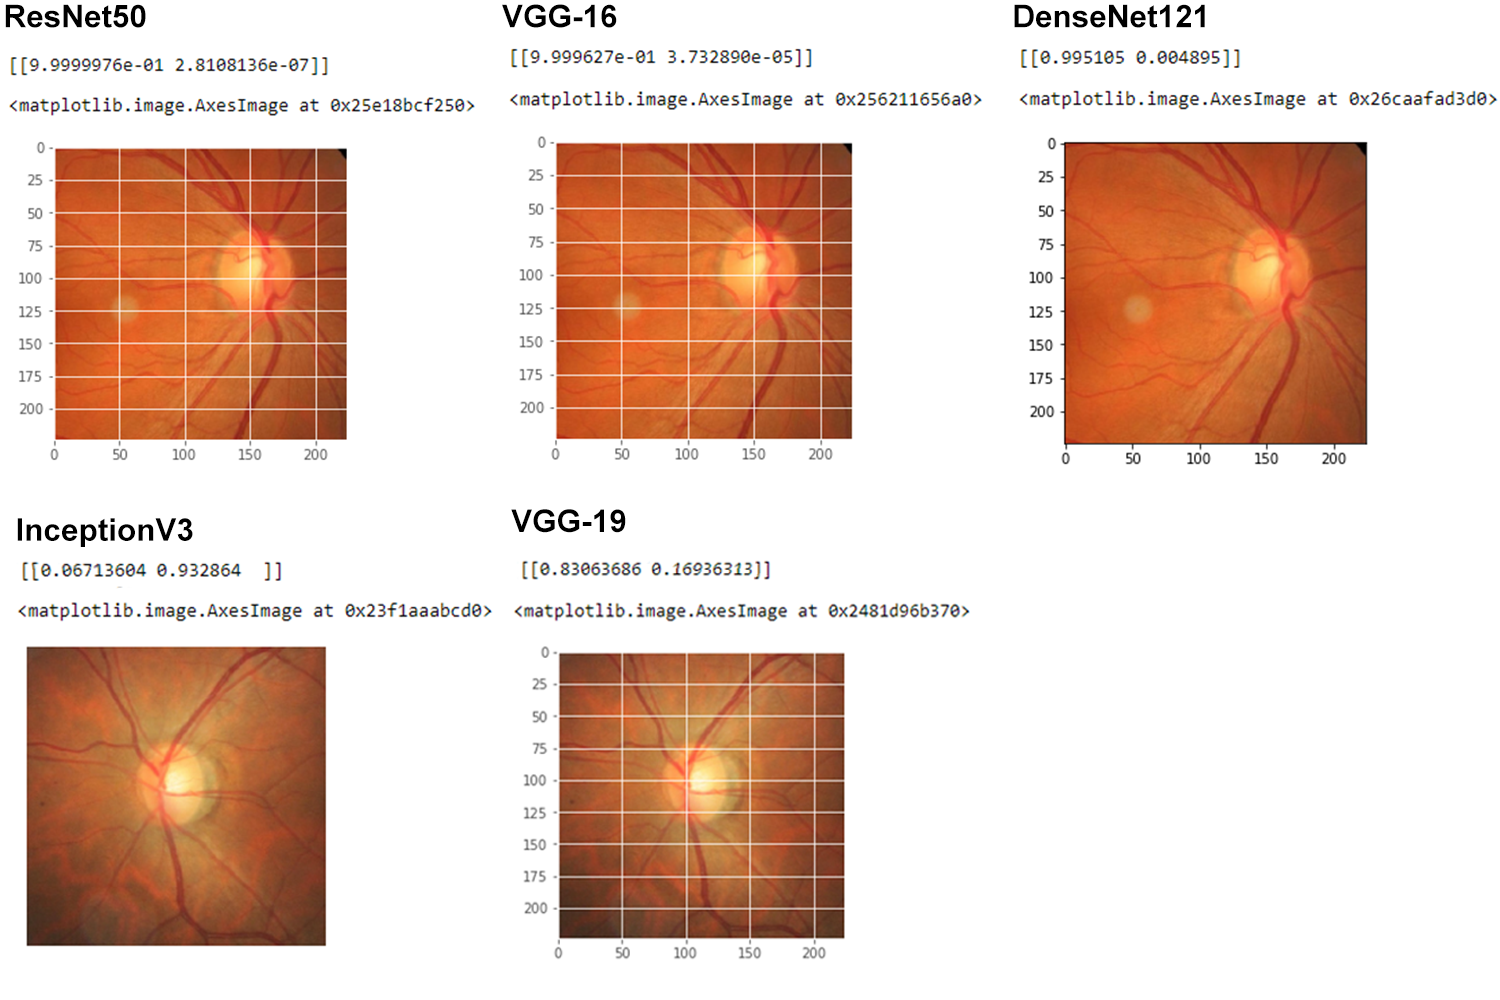
\includegraphics[scale=0.6]{images/fig-53.png}
\caption{Single Image Predictions for all Model}
\label{fig:x Single Image Predictions for all Model}
\end{figure}

\newpage
\vspace{5mm}
\noindent\textit{These are batch (50 images/batch) image predictions of all models - ( here [1,0] means glaucoma and [0,1] means non-glaucoma )}


\vspace{5mm}
\begin{figure}[hbt!]
\centering
\includegraphics[scale=0.6]{images/fig-54.png}
\caption{Batch Predictions for DenseNet121}
\label{fig:x Batch Predictions for DenseNet121}
\end{figure}

\vspace{5mm}
\begin{figure}[hbt!]
\centering
\includegraphics[scale=0.6]{images/fig-55.png}
\caption{Batch Predictions for InceptionV3}
\label{fig:x Batch Predictions for InceptionV3}
\end{figure}

\newpage
\vspace{5mm}
\noindent\textit{These are batch (50 images/batch) image predictions of all models - ( here [1,0] means glaucoma and [0,1] means non-glaucoma )}

\vspace{5mm}
\begin{figure}[hbt!]
\centering
\includegraphics[scale=0.6]{images/fig-56.png}
\caption{Batch Predictions for VGG-16}
\label{fig:x Batch Predictions for VGG-16}
\end{figure}

\vspace{5mm}
\begin{figure}[hbt!]
\centering
\includegraphics[scale=0.6]{images/fig-57.png}
\caption{Batch Predictions for VGG-19}
\label{fig:x Batch Predictions for VGG-19}
\end{figure}

\vspace{5mm}
\begin{figure}[hbt!]
\centering
\includegraphics[scale=0.6]{images/fig-58.png}
\caption{ Batch Predictions for ResNet50}
\label{fig:x  Batch Predictions for ResNet50}
\end{figure}



\nomenclature{$OOP$}{Object Oriented Programming}
\nomenclature{$AdaM$}{Adaptive Momentum}
